\documentclass[12pt,a4paper,portrait]{article}
%\setcounter{secnumdepth}{0}
\usepackage{gensymb}
\usepackage{pdflscape}
\usepackage{amsmath}
\usepackage{amssymb}
\usepackage{enumitem}
\usepackage{graphicx}
\usepackage{subcaption}
\usepackage{multirow}
\usepackage{sansmath}
\usepackage{pst-eucl}
\usepackage{multicol}
\usepackage{csquotes}
% Coding
\usepackage{listings}
\setlength{\parindent}{0pt}
\usepackage[obeyspaces]{url}
% Better inline directory listings
\usepackage{xcolor}
\definecolor{light-gray}{gray}{0.95}
\newcommand{\code}[1]{\colorbox{light-gray}{\texttt{#1}}}
\usepackage{adjustbox}
\usepackage[UKenglish]{isodate}
\usepackage[UKenglish]{babel}
\usepackage{float}
\usepackage[T1]{fontenc}
\usepackage{setspace}
\usepackage{sectsty}
\usepackage{longtable}
\newenvironment{tightcenter}{%
	\setlength\topsep{0pt}
	\setlength\parskip{0pt}
	\begin{center}
	}{%
	\end{center}
}
\captionsetup{width=\textwidth}
\usepackage{mbenotes} % to print table notes!
\usepackage{alphalph} % For extended counters!
% usage: \tabnotemark[3]\cmsp\tabnotemark[4]
\usepackage[colorlinks=true,linkcolor=blue,urlcolor=black,bookmarksopen=true]{hyperref}
\sectionfont{%			            % Change font of \section command
	\usefont{OT1}{phv}{b}{n}%		% bch-b-n: CharterBT-Bold font
	\sectionrule{0pt}{0pt}{-5pt}{3pt}}
\subsectionfont{
	\usefont{OT1}{phv}{b}{n}}
\newcommand{\MyName}[1]{ % Name
	\usefont{OT1}{phv}{b}{n} \begin{center}of {\LARGE  #1}\end{center}
	\par \normalsize \normalfont}
\makeatletter
\newcommand\FirstWord[1]{\@firstword#1 \@nil}%
\newcommand\@firstword{}%
\newcommand\@removecomma{}%
\def\@firstword#1 #2\@nil{\@removecomma#1,\@nil}%
\def\@removecomma#1,#2\@nil{#1}
\makeatother

\newcommand{\MyTitle}[1]{ % Name
	\Huge \usefont{OT1}{phv}{b}{n} \begin{center}#1\end{center}
	\par \normalsize \normalfont}
\newcommand{\lag}{\mathcal{L}}
\newcommand{\ham}{\mathcal{H}}
\newcommand{\eq}[1]{Equation \eqref{#1}}
\newcommand{\NewPart}[1]{\section*{\uppercase{#1}}}
\newcommand{\NewSubPart}[1]{\subsection*{\hspace{0.2cm}#1}}
\renewcommand{\baselinestretch}{1.05}
\usepackage[margin=0.2cm]{geometry}
\date{}
\title{Elastic pendula}
\author{Brenton Horne}

\begin{document}
\maketitle

In this document, we will go over classical mechanical problems that involve an elastic pendulum. An elastic pendulum is one whose rod instead of being rigid is an elastic spring. This complicates the calculation by making the length of the pendulum rod variable instead of fixed and adding an extra force to the system (the spring force). Friction forces will be accounted for using linear and quadratic (of velocity) terms. 
\tableofcontents

\section{Preliminaries}
There are a few classical mechanical formalisms we could use to derive the equations of motion for elastic pendulum systems with friction. Newtonian mechanics is one approach, but this approach uses vectors and is unnecessarily complicated. Alternatively, Lagrangian and Hamiltonian mechanics could provide a simpler path to a solution. Of these, Lagrangian mechanics is likely simpler, as using the Hamiltonian approach would require us to write the kinetic energy in terms of generalized momenta ($p_i$), which will take some work. Hamiltonian mechanics usually makes up for this by providing ordinary differential equation (ODE) systems that can be integrated using symplectic methods. These methods minimize the accumulation of errors in the Hamiltonian of the system over time. 

\subsection{Lagrangian formalism}
In Lagrangian mechanics, the equations of motion are the Euler-Lagrange equations, which are in terms of the Lagrangian --- $\lag$ --- which is the kinetic and potential energy difference. These equations can be written, with a dissipative force, as
\begin{align}
	\dfrac{d}{dt}\left(\dfrac{\partial \lag}{\partial \dot{q}_i}\right) - \dfrac{\partial \lag}{\partial q_i} &= Q_i. \label{ELD}
\end{align}

Where $Q_i$ is the generalized dissipative force, which is defined as
\begin{align}
	Q_i &= \sum_{j} \vec{F}_{D,j} \cdot \hat{e}_{j,i}.\label{GDF}
\end{align}

Where $\vec{F}_{D,j}$ is the dissipative force vector for particle $j$. In \eq{GDF}, $\hat{e}_{j,i}$ is the generalized basis vector of particle $j$ and generalized coordinate $q_i$. In this case, our generalized coordinates $q_i$ would consist of $\theta$ and $z$. The generalized basis vectors are defined as
\begin{align*}
	\hat{e}_{j,i} &= \dfrac{\partial \vec{r}_j}{\partial q_i}.
\end{align*}
 
\subsection{Hamiltonian formalism}
As for the Hamiltonian formalism, the equations of motion there are

\begin{align}
	\dot{q}_i &= \dfrac{\partial \ham}{\partial p_i} \label{qdoti}\\
	\dot{p}_i &= -\dfrac{\partial \ham}{\partial q_i} + Q_i. \label{pdoti}
\end{align}

Where $\ham$ is the kinetic energy plus potential energy. 

\section{Single elastic pendulum with friction}
Say we have a mass $m$ attached to a spring of rest length $l$. Suppose we call the displacement from rest $z$. That way the length of the spring is $l(t) = l + z$. Let us measure  $\theta$ clockwise from the positive x-axis.

\subsection{Position and velocity}
The Cartesian coordinates of the pendulum bob are defined as

\begin{align*}
	x &= (l+z)\cos{\theta} &\implies \dot{x} &= \dot{z}\cos{\theta} - (l+z)\dot{\theta}\sin{\theta}\\
	y &= (l+z)\sin{\theta} &\implies \dot{y} &= \dot{z}\sin{\theta} + (l+z)\dot{\theta}\cos{\theta}.\\
\end{align*}

Velocity is given by

\begin{align*}
	\vec{v} &= \begin{bmatrix}
		\dot{z}\cos{\theta} - (l+z)\dot{\theta}\sin{\theta} \\
		\dot{z}\sin{\theta} + (l+z)\dot{\theta}\cos{\theta}
	\end{bmatrix}\\
	|\vec{v}_1|^2 &= |\vec{v}_1|^2 \\
	&= \dot{x}^2+\dot{y}^2 \\
	&= \left[\dot{z}\cos{\theta} - (l+z)\dot{\theta}\sin{\theta}\right]^2 + \left[\dot{z}\sin{\theta} + (l+z)\dot{\theta}\cos{\theta}\right]^2 \\
	&= \dot{z}^2 \cos^2{\theta} + (l+z)^2\dot{\theta}^2\sin^2{\theta} - 2\dot{z}\dot{\theta}(l+z)\cos{\theta}\sin{\theta} + \dot{z}^2\sin^2{\theta} + (l+z)^2\dot{\theta}^2\cos^2{\theta} + 2\dot{z}\dot{\theta}(l+z)\sin{\theta}\cos{\theta} \\
	&= \dot{z}^2 + (l+z)^2\dot{\theta}^2\\
\therefore |\vec{v}| &= \sqrt{|\vec{v}_1|^2}\\
	&= \sqrt{\dot{z}^2+(l+z)^2\dot{\theta}^2}.
\end{align*}

\subsection{Generalized basis vector}
Next we will calculate $\dfrac{\partial \vec{r}}{\partial q_i}$

\begin{align*}
	\dfrac{\partial \vec{r}}{\partial \theta} &= (l+z)\begin{bmatrix}
		-\sin{\theta} \\
		\cos{\theta}
	\end{bmatrix} \\
	\dfrac{\partial \vec{r}}{\partial z} &= \begin{bmatrix}
		\cos{\theta} \\
		\sin{\theta}
	\end{bmatrix}.
\end{align*}

\subsection{Kinetic energy}
Hence the kinetic energy is
\begin{align*}
	T &= \dfrac{m|\vec{v}_1|^2}{2} \\
	&= \dfrac{m}{2} \left[\dot{z}^2 + (l+z)^2\dot{\theta}^2\right].
\end{align*}

\subsection{Potential energy}
As for the potential energy, it will have two components: a spring component,
\begin{align*}
	V_S &= \dfrac{kz^2}{2};
\end{align*}

and a graphical component,
\begin{align*}
	V_G &= mgy \\
	&= mg(l+z)\sin{\theta}.
\end{align*}

Therefore the total potential energy is
\begin{align*}
	V &= V_S + V_G \\
	&= \dfrac{kz^2}{2} + mg(l+z)\sin{\theta}.
\end{align*}

\subsection{Lagrangian}
Hence the Lagrangian is
\begin{align*}
	\lag &= T - V \\
	&= \dfrac{m}{2} \left[\dot{z}^2 + \dot{\theta}^2(l+z)^2\right] - \dfrac{kz^2}{2} - mg(l+z)\sin{\theta}.
\end{align*}

\subsection{Dissipative forces}
What dissipative forces should be included? Let us include linear and quadratic in velocity terms to account for air resistance and other forms of friction. 

\begin{align*}
	\vec{F}_D &= -b\vec{v} - c|\vec{v}|\vec{v}.
\end{align*}

We have already calculate the components of the velocity vector---they are $\dot{x}$ and $\dot{y}$, respectively. 

\begin{align*}
	\vec{v} &= \begin{bmatrix}
		\dot{z}\cos{\theta} - (l+z)\dot{\theta}\sin{\theta} \\
		\dot{z}\sin{\theta} + (l+z)\dot{\theta}\cos{\theta}
	\end{bmatrix}\\
	|\vec{v}| &= \sqrt{|\vec{v}_1|^2}\\
	&= \sqrt{\dot{z}^2+(l+z)^2\dot{\theta}^2}.
\end{align*}

To calculate, $Q_i$ we must find $\vec{v} \cdot \dfrac{\partial \vec{r}}{\partial q_i}$

\begin{align*}
	\vec{v} \cdot \dfrac{\partial \vec{r}}{\partial \theta} &= \begin{bmatrix}
		\dot{z}\cos{\theta} - (l+z)\dot{\theta}\sin{\theta} \\
		\dot{z}\sin{\theta} + (l+z)\dot{\theta}\cos{\theta}
	\end{bmatrix} \cdot (l+z)\begin{bmatrix}
		-\sin{\theta} \\
		\cos{\theta}
	\end{bmatrix} \\
	&= -\dot{z}(l+z)\cos{\theta} \sin{\theta} + (l+z)^2 \dot{\theta}\sin^2{\theta} + \dot{z}(l+z)\sin{\theta} \cos{\theta} +(l+z)^2\dot{\theta}\cos^2{\theta} \\
	&= (l+z)^2 \dot{\theta} \\
	\vec{v} \cdot \dfrac{\partial \vec{r}}{\partial z} &= \begin{bmatrix}
		\dot{z}\cos{\theta} - (l+z)\dot{\theta}\sin{\theta} \\
		\dot{z}\sin{\theta} + (l+z)\dot{\theta}\cos{\theta}
	\end{bmatrix} \cdot \begin{bmatrix}
		\cos{\theta} \\
		\sin{\theta}
	\end{bmatrix} \\
	&= \dot{z}\cos^2{\theta} - (l+z)\dot{\theta} \sin{\theta}\cos{\theta} + \dot{z}\sin^2{\theta} + (l+z)\dot{\theta}\cos{\theta}\sin{\theta} \\
	&= \dot{z}. 
\end{align*}

Hence $Q_i$ is

\begin{align*}
	Q_{\theta} &= -(l+z)^2 \dot{\theta} \left(b+c\sqrt{\dot{z}^2+(l+z)^2\dot{\theta}^2}\right) \\
	Q_z &= -\dot{z}\left(b+c\sqrt{\dot{z}^2+(l+z)^2\dot{\theta}^2}\right).
\end{align*}

\subsection{Left-hand side of \eq{ELD}}
\subsubsection{$\theta$}
As for the LHS of \eq{ELD}, let us work on it for $\theta$ one term at a time
\begin{align*}
	p_{\theta} &= \dfrac{\partial \lag}{\partial \dot{\theta}} \\
	&= m\dot{\theta}(l+z)^2 \\
	\dot{p_{\theta}} &= m\ddot{\theta} (l+z)^2 + 2m\dot{\theta}\dot{z}(l+z) \\
	F_{\theta} &= \dfrac{\partial \lag}{\partial \theta} \\
	&= -mg(l+z)\cos{\theta}.
\end{align*}

Substituting into \eq{ELD} yields
\begin{align*}
	m\ddot{\theta} (l+z)^2 + 2m\dot{\theta}\dot{z}(l+z) - (-mg(l+z)\cos{\theta}) &= -(l+z)^2 \dot{\theta} \left(b+c\sqrt{\dot{z}^2+(l+z)^2\dot{\theta}^2}\right) \\
	m\ddot{\theta} (l+z)^2 + 2m\dot{\theta}\dot{z}(l+z) +mg(l+z)\cos{\theta} &= -(l+z)^2 \dot{\theta} \left(b+c\sqrt{\dot{z}^2+(l+z)^2\dot{\theta}^2}\right) \\
	\ddot{\theta} &= -\dfrac{2\dot{\theta}\dot{z}}{l+z} - \dfrac{g\cos{\theta}}{l+z} -\dfrac{\dot{\theta}}{m} \left(b+c\sqrt{\dot{z}^2+(l+z)^2\dot{\theta}^2}\right). \\
\end{align*}

Let $k'=\dfrac{k}{m}$, $b'=\dfrac{b}{m}$ and $c'=\dfrac{c}{m}$.

\begin{align*}
	\ddot{\theta} &= -\dfrac{2\dot{\theta}\dot{z}}{l+z} - \dfrac{g\cos{\theta}}{l+z} -\dot{\theta} \left(b'+c'\sqrt{\dot{z}^2+(l+z)^2\dot{\theta}^2}\right).
\end{align*}

\subsubsection{$z$}
As for $z$

\begin{align*}
	p_z &= \dfrac{\partial \lag}{\partial \dot{z}} \\
	&= m\dot{z} \\
	\dot{p_z} &= m\ddot{z} \\
	F_z &= \dfrac{\partial \lag}{\partial z} \\
	&= m\dot{\theta}^2(l+z) - kz - mg\sin{\theta}.
\end{align*}

Substituting into \eq{ELD} yields

\begin{align*}
	m\ddot{z} - m\dot{\theta}^2(l+z) + kz + mg\sin{\theta} &= -\dot{z}\left(b+c\sqrt{\dot{z}^2+(l+z)^2\dot{\theta}^2}\right) \\
	\ddot{z} &= \dot{\theta}^2(l+z) - \dfrac{kz}{m} - g\sin{\theta} -\dfrac{\dot{z}}{m}\left(b+c\sqrt{\dot{z}^2+(l+z)^2\dot{\theta}^2}\right).
\end{align*}

Let $k'=\dfrac{k}{m}$, $b'=\dfrac{b}{m}$ and $c'=\dfrac{c}{m}$.

\begin{align*}
	\ddot{z} &= \dot{\theta}^2(l+z) - k'z - g\sin{\theta} -\dot{z}\left(b'+c'\sqrt{\dot{z}^2+(l+z)^2\dot{\theta}^2}\right).
\end{align*}

\subsection{Hamiltonian mechanics}
First, we will rewrite $\vec{v}$ and $|\vec{v}_1|^2$ in terms of $p_{\theta}$ and $p_z$. 

\begin{align*}
	\vec{v} &= \dfrac{1}{m}\begin{bmatrix}
		p_z\cos{\theta} - \dfrac{p_{\theta}\sin{\theta}}{l+z}\\
		p_z\sin{\theta} + \dfrac{p_{\theta}\cos{\theta}}{l+z}
	\end{bmatrix} \\
	|\vec{v}_1|^2 &= \dot{z}^2 + (l+z)^2 \dot{\theta}^2 \\
	&= \dfrac{p_z^2}{m^2} + \dfrac{p_{\theta}^2}{m^2(l+z)^2}.
\end{align*}

Hence the kinetic energy is

\begin{align*}
	T &= \dfrac{m}{2} |\vec{v}_1|^2 \\
	&= \dfrac{p_z^2}{2m} + \dfrac{p_{\theta}^2}{2m(l+z)^2},
\end{align*}

the Hamiltonian is

\begin{align*}
	\ham &= T + V\\
	&= \dfrac{p_z^2}{2m} + \dfrac{p_{\theta}^2}{2m(l+z)^2} + \dfrac{kz^2}{2} + mg(l+z)\sin{\theta},
\end{align*}

and the generalized dissipative forces are

\begin{align*}
	Q_z &= -\dfrac{p_z}{m}\left(b+c\sqrt{\dfrac{p_z^2}{m^2} + \dfrac{p_{\theta}^2}{m^2(l+z)^2}}\right) \\
	Q_{\theta} &= -\dfrac{p_{\theta}}{m} \left(b+c\sqrt{\dfrac{p_z^2}{m^2} + \dfrac{p_{\theta}^2}{m^2(l+z)^2}}\right).
\end{align*}

\subsubsection{$z$}
\begin{align*}
	\dot{z} &= \dfrac{\partial \ham}{\partial p_z} \\
	&= \dfrac{p_z}{m} \\
	\dot{p}_z &= -\dfrac{\partial \ham}{\partial z} + Q_z\\
	&= \dfrac{p_{\theta}^2}{m(l+z)^3} - kz - mg\sin{\theta} + Q_z
\end{align*}

\subsubsection{$\theta$}
\begin{align*}
	\dot{\theta} &= \dfrac{\partial \ham}{\partial p_{\theta}} \\
	&= \dfrac{p_{\theta}}{m(l+z)^2} \\
	\dot{p}_{\theta} &= -\dfrac{\partial \ham}{\partial \theta} + Q_{\theta} \\
	&= -mg(l+z)\cos{\theta} + Q_{\theta}.
\end{align*}

\section{Elastic spherical pendulum}
Here we have a single elastic pendulum whose bob position is described in spherical coordinates. We will not provide a diagram as drawing in 3D is a bit more challenging.

\subsection{Coordinates}
\begin{align*}
	x &= r\cos{\theta}\sin{\varphi}\\
	y &= r\sin{\theta}\sin{\varphi} \\
	z &= r\cos{\varphi}.
\end{align*}

Where $r = l + \xi$. Here $l$ is the rest length of the pendulum rods and $\xi$ is the displacement of them. 

\begin{landscape}
\subsection{Velocity}
Hence our velocity vector is

\begin{align*}
	\vec{v} &= \dfrac{d}{dt}{\vec{r}} \\
	&= \begin{bmatrix}
		\dot{r}\cos{\theta}\sin{\varphi}  - r\dot{\theta}\sin{\theta}\sin{\varphi} + r\dot{\varphi}\cos{\theta}\cos{\varphi} \\
		\dot{r}\sin{\theta}\sin{\varphi}  + r\dot{\theta}\cos{\theta}\sin{\varphi} + r\dot{\varphi}\sin{\theta}\cos{\varphi} \\
		\dot{r}\cos{\varphi} - r\dot{\varphi}\sin{\varphi}
	\end{bmatrix} \\
	|\vec{v}|^2 &= \dot{r}^2\cos^2{\theta}\sin^2{\varphi}  + r^2\dot{\theta}^2\sin^2{\theta}\sin^2{\varphi} + r^2\dot{\varphi}^2\cos^2{\theta}\cos^2{\varphi} - 2\dot{r}r\dot{\theta}\cos{\theta}\sin{\theta}\sin^2{\varphi} + 2\dot{r}r\dot{\varphi}\cos^2{\theta}\sin{\varphi}\cos{\varphi} - 2r^2\dot{\theta}\dot{\varphi}\sin{\theta}\cos{\theta}\sin{\varphi}\cos{\varphi} + \dot{r}^2\sin^2{\theta}\sin^2{\varphi}  \\
	&+ r^2\dot{\theta}^2\cos^2{\theta}\sin^2{\varphi} + r^2\dot{\varphi}^2\sin^2{\theta}\cos^2{\varphi} + 2r\dot{r}\dot{\theta}\sin{\theta}\cos{\theta}\sin^2{\varphi} + 2r\dot{r}\dot{\varphi}\sin^2{\theta}\sin{\varphi}\cos{\varphi} + 2r^2\dot{\theta}\dot{\varphi}\sin{\theta}\cos{\theta}\sin{\varphi}\cos{\varphi} + \dot{r}^2\cos^2{\varphi} + r^2\dot{\varphi}^2\sin^2{\varphi} - 2r\dot{r}\dot{\varphi}\cos{\varphi}\sin{\varphi}\\
	&= \dot{r}^2 + r^2\dot{\theta}^2\sin^2{\varphi} + r^2\dot{\varphi}^2 \\
	\therefore |\vec{v}| &= \sqrt{\dot{r}^2 + r^2\dot{\theta}^2\sin^2{\varphi} + r^2\dot{\varphi}^2}.
\end{align*}

\subsection{Lagrangian}
Hence the Lagrangian is

\begin{align*}
	\lag &= \dfrac{m|\vec{v}|^2}{2} - mgz - \dfrac{k\xi^2}{2} \\
	&= \dfrac{m|\vec{v}|^2}{2} - mgr\cos{\varphi} - \dfrac{k(r-l)^2}{2}.
\end{align*}

\subsection{Euler-Lagrange equations with dissipation}
\subsubsection{Length of pendulum: $r$}
Hence \eq{ELD} for $r$ has the components

\begin{align*}
	\dfrac{\partial \lag}{\partial r} &= m(r\dot{\theta}^2\sin^2{\varphi} + r\dot{\varphi}^2-g\cos{\varphi}) - k(r-l) \\
	\dfrac{\partial \lag}{\partial \dot{r}} &= m\dot{r} \\
	\dfrac{d}{dt} \dfrac{\partial \lag}{\partial \dot{r}} &= m\ddot{r}.
\end{align*}
Consequently, the functional derivative of $\lag$ with respect to $r$ is
\begin{align*}
	\dfrac{\delta \lag}{\delta r} &= \dfrac{d}{dt} \dfrac{\partial \lag}{\partial \dot{r}} -\dfrac{\partial \lag}{\partial r} \\
	&= m\ddot{r} - \left[m(r\dot{\theta}^2\sin^2{\varphi} + r\dot{\varphi}^2-g\cos{\varphi}) - k(r-l)\right] \\
	&= m\left[\ddot{r} - r\dot{\theta}^2\sin^2{\varphi} - r\dot{\varphi}^2+g\cos{\varphi}\right] + k(r-l).
\end{align*}

The dissipation term is
\begin{align*}
	Q_r &= -(b + c|\vec{v}|)\vec{v} \cdot \dfrac{\partial \vec{r}}{\partial r} \\
	&= -(b + c|\vec{v}|) \begin{bmatrix}
		\dot{r}\cos{\theta}\sin{\varphi}  - r\dot{\theta}\sin{\theta}\sin{\varphi} + r\dot{\varphi}\cos{\theta}\cos{\varphi} \\
		\dot{r}\sin{\theta}\sin{\varphi}  + r\dot{\theta}\cos{\theta}\sin{\varphi} + r\dot{\varphi}\sin{\theta}\cos{\varphi} \\
		\dot{r}\cos{\varphi} - r\dot{\varphi}\sin{\varphi}
	\end{bmatrix} \cdot \begin{bmatrix}
	\cos{\theta}\sin{\varphi}\\
	\sin{\theta}\sin{\varphi} \\
	\cos{\varphi}
	\end{bmatrix} \\
	&= -(b + c|\vec{v}|) \left[\dot{r}\cos^2{\theta}\sin^2{\varphi} - r\dot{\theta}\sin{\theta}\cos{\theta}\sin^2{\varphi} + r\dot{\varphi}\cos^2{\theta}\sin{\varphi}\cos{\varphi} + \dot{r}\sin^2{\theta}\sin^2{\varphi} + r\dot{\theta}\sin{\theta}\cos{\theta}\sin^2{\varphi} + r\dot{\varphi}\sin^2{\theta}\cos{\varphi}\sin{\varphi} + \dot{r}\cos^2{\varphi} - r\dot{\varphi}\cos{\varphi}\sin{\varphi}\right]\\
	&= -(b + c|\vec{v}|)\dot{r}.
\end{align*}

Hence the Euler-Lagrange equation with dissipation for $r$ is

\begin{align*}
	m\left[\ddot{r} - r\dot{\theta}^2\sin^2{\varphi} - r\varphi^2+g\cos{\varphi}\right] + k(r-l) &= -(b + c|\vec{v}|)\dot{r} \\
	\ddot{r} - r\dot{\theta}^2\sin^2{\varphi} - r\varphi^2+g\cos{\varphi} + \dfrac{k}{m}(r-l) &= \dfrac{-(b + c|\vec{v}|)\dot{r}}{m} \\
	\ddot{r} &= r\dot{\theta}^2\sin^2{\varphi} + r\varphi^2 - g\cos{\varphi} - \dfrac{(b + c|\vec{v}|)\dot{r}+k(r-l)}{m}.
\end{align*}

\subsubsection{Angle pendulum makes with positive $x$-axis: $\theta$}
As for $\theta$

\begin{align*}
	\dfrac{\partial \lag}{\partial \theta} &= 0 \\
	\dfrac{\partial \lag}{\partial \dot{\theta}} &= mr^2\dot{\theta}\sin^2{\varphi} \\
	\dfrac{d}{dt} \dfrac{\partial \lag}{\partial \dot{\theta}} &= mr^2\ddot{\theta} \sin^2{\varphi} + 2mr\dot{r}\dot{\theta}\sin^2{\varphi} + mr^2\dot{\theta}\dot{\varphi}\sin{2\varphi} \\
	\dfrac{\delta \lag}{\delta \theta} &= mr^2\ddot{\theta} \sin^2{\varphi} + 2mr\dot{r}\dot{\theta}\sin^2{\varphi} + mr^2\dot{\theta}\dot{\varphi}\sin{2\varphi} \\
	Q_{\theta} &= -(b+c|\vec{v}|)\vec{v} \cdot \dfrac{\partial \vec{r}}{\partial \theta} \\
	&= -(b+c|\vec{v}|) \begin{bmatrix}
		\dot{r}\cos{\theta}\sin{\varphi}  - r\dot{\theta}\sin{\theta}\sin{\varphi} + r\dot{\varphi}\cos{\theta}\cos{\varphi} \\
		\dot{r}\sin{\theta}\sin{\varphi}  + r\dot{\theta}\cos{\theta}\sin{\varphi} + r\dot{\varphi}\sin{\theta}\cos{\varphi} \\
		\dot{r}\cos{\varphi} - r\dot{\varphi}\sin{\varphi}
	\end{bmatrix} \cdot \begin{bmatrix}
	-r\sin{\theta}\sin{\varphi} \\
	r\cos{\theta}\sin{\varphi} \\
	0
\end{bmatrix} \\
&= -(b+c|\vec{v}|)\left[-r\dot{r}\cos{\theta}\sin{\theta}\sin^2{\varphi} + r^2\dot{\theta}\sin^2{\theta}\sin^2{\varphi} - r^2\dot{\varphi}\sin{\theta}\cos{\theta}\cos{\varphi}\sin{\varphi} + r\dot{r}\sin{\theta}\cos{\theta}\sin^2{\varphi} + r^2\dot{\theta}\cos^2{\theta}\sin^2{\varphi} + r^2\dot{\varphi}\sin{\theta}\cos{\theta}\cos{\varphi}\sin{\varphi}\right]\\
&= -(b+c|\vec{v}|)r^2\dot{\theta}\sin^2{\varphi}.
\end{align*}

Hence \eq{ELD} for $\theta$ is

\begin{align*}
	mr^2\ddot{\theta} \sin^2{\varphi} + 2mr\dot{r}\dot{\theta}\sin^2{\varphi} + mr^2\dot{\theta}\dot{\varphi}\sin{2\varphi} &= -(b+c|\vec{v}|)r^2\dot{\theta}\sin^2{\varphi}.
\end{align*}

Dividing by $mr^2\sin^2{\varphi}$ yields

\begin{align*}
	\ddot{\theta} + \dfrac{2\dot{r}\dot{\theta}}{r} + 2\dot{\theta}\dot{\varphi}\cot{\varphi} &= -\dfrac{(b+c|\vec{v}|)\dot{\theta}}{m} \\
	\ddot{\theta} &= -\dfrac{2\dot{r}\dot{\theta}}{r} - 2\dot{\theta}\dot{\varphi}\cot{\varphi} -\dfrac{(b+c|\vec{v}|)\dot{\theta}}{m}.
\end{align*}

Which will sadly be unstable whenever $\varphi \approx n\pi$ where $n\in \mathbb{Z}$.

\subsubsection{Angle pendulum makes with positive $z$-axis: $\varphi$}
As for $\varphi$

\begin{align*}
	\dfrac{\partial \lag}{\partial \varphi} &= \dfrac{mr^2\dot{\theta}^2\sin{2\varphi}}{2} + mgr\sin{\varphi} \\
	\dfrac{\partial \lag}{\partial \dot{\varphi}} &= mr^2\dot{\varphi} \\
	\dfrac{d}{dt}\dfrac{\partial \lag}{\partial \dot{\varphi}} &= 2mr\dot{r}\dot{\varphi} + mr^2 \ddot{\varphi} \\
	\dfrac{\delta \lag}{\partial \varphi} &= 2mr\dot{r}\dot{\varphi} + mr^2 \ddot{\varphi} -\left[ \dfrac{mr^2\dot{\theta}^2\sin{2\varphi}}{2} + mgr\sin{\varphi}\right] \\
	&= mr^2\left[\ddot{\varphi} + \dfrac{2\dot{r}\dot{\varphi}}{r} - \dfrac{\dot{\theta}^2\dot{\varphi}\sin{2\varphi}}{2} -\dfrac{g\sin{\varphi}}{r} \right]\\
	Q_{\varphi} &= -(b+c|\vec{v}|) \begin{bmatrix}
		\dot{r}\cos{\theta}\sin{\varphi}  - r\dot{\theta}\sin{\theta}\sin{\varphi} + r\dot{\varphi}\cos{\theta}\cos{\varphi} \\
		\dot{r}\sin{\theta}\sin{\varphi}  + r\dot{\theta}\cos{\theta}\sin{\varphi} + r\dot{\varphi}\sin{\theta}\cos{\varphi} \\
		\dot{r}\cos{\varphi} - r\dot{\varphi}\sin{\varphi}
	\end{bmatrix} \cdot \begin{bmatrix}
	r\cos{\theta}\cos{\varphi} \\
	r\sin{\theta}\cos{\varphi} \\
	-r\sin{\varphi}
	\end{bmatrix} \\
	&= -(b+c|\vec{v}|)\left[r\dot{r}\cos^2{\theta}\cos{\varphi}\sin{\varphi} - r^2\dot{\theta}\sin{\theta}\cos{\theta}\sin{\varphi}\cos{\varphi} + r^2\dot{\varphi}\cos^2{\theta}\cos^2{\varphi} + r\dot{r}\sin^2{\theta}\sin{\varphi}\cos{\varphi} + r^2\dot{\theta}\cos{\theta}\sin{\theta}\cos{\varphi}\sin{\varphi} + r^2 \dot{\varphi}\sin^2{\theta}\cos^2{\varphi}  - r\dot{r}\cos{\varphi}\sin{\varphi} \right.\\
	&\left.+ r^2\dot{\varphi}\sin^2{\varphi}\right] \\
	&= -(b+c|\vec{v}|)r^2\dot{\varphi}.
\end{align*}

Hence \eq{ELD} for $\varphi$ is

\begin{align*}
	mr^2\left[\ddot{\varphi} + \dfrac{2\dot{r}\dot{\varphi}}{r} - \dfrac{\dot{\theta}^2\sin{2\varphi}}{2} -\dfrac{g\sin{\varphi}}{r} \right] &= -(b+c|\vec{v}|)r^2\dot{\varphi} \\
	\ddot{\varphi} + \dfrac{2\dot{r}\dot{\varphi}}{r} - \dfrac{\dot{\theta}^2\sin{2\varphi}}{2} -\dfrac{g\sin{\varphi}}{r} &= -\dfrac{(b+c|\vec{v}|)\dot{\varphi}}{m} \\
	\ddot{\varphi} &= \dfrac{g\sin{\varphi} - 2\dot{r}\dot{\varphi}}{r} + \dot{\theta}^2\sin{\varphi}\cos{\varphi} - \dfrac{(b+c|\vec{v}|)\dot{\varphi}}{m}.
\end{align*}

\end{landscape}
\section{Cart with elastic pendulum}
\begin{figure}[H]
	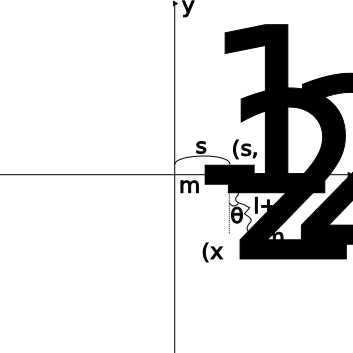
\includegraphics[width=500px]{Elastic pendulum on a cart.png}
	\caption{Diagram of problem.}\label{fig1}
\end{figure}

Here we have a cart whose centre of mass is at $(s, 0)$ and a pendulum attached to its horizontal centre bottom. To simplify calculations, we will assume the height of the cart is 0, but adding a constant height to the cart will not change the equations of motion.

\subsection{Coordinates, velocity and kinetic energy}
Hence the kinetic energy for the cart is $\dfrac{m_1}{2}\dot{s}^2$. Next, we will calculate the coordinates, velocity and kinetic energy of the pendulum

\begin{align*}
	x_2 &= s + (l+z)\sin{\theta} \\
	\dot{x}_2 &= \dot{s} + \dot{z}\sin{\theta} + (l+z)\dot{\theta}\cos{\theta}\\
	y_2 &= -(l+z)\cos{\theta} \\
	\dot{y}_2 &= -\dot{z}\cos{\theta} + (l+z)\dot{\theta}\sin{\theta} \\
	v_2^2 &= \dot{x}_2^2 + \dot{y}_2^2 \\
	&= (\dot{s} + \dot{z}\sin{\theta} + (l+z)\dot{\theta}\cos{\theta})^2 + (-\dot{z}\cos{\theta} + (l+z)\dot{\theta}\sin{\theta})^2 \\
	&= \dot{s}^2 + \dot{z}^2 \sin^2{\theta} + (l+z)^2\dot{\theta}^2\cos^2{\theta} + 2\dot{s}\dot{z}\sin{\theta} + 2\dot{s}\dot{\theta}(l+z)\cos{\theta} + 2\dot{z}\dot{\theta}(l+z)\sin{\theta}\cos{\theta} + \dot{z}^2\cos^2{\theta} \\
	&+ (l+z)^2\dot{\theta}^2\sin^2{\theta} - 2\dot{z}\dot{\theta}(l+z)\cos{\theta}\sin{\theta}\\
	&= \dot{s}^2 + \dot{z}^2 + (l+z)^2\dot{\theta}^2 + 2\dot{s}(\dot{z}\sin{\theta} + \dot{\theta}(l+z)\cos{\theta})\\
	T_p &= \dfrac{m_2}{2} \left(\dot{s}^2 + \dot{z}^2 + (l+z)^2\dot{\theta}^2 + 2\dot{s}(\dot{z}\sin{\theta} + \dot{\theta}(l+z)\cos{\theta})\right).
\end{align*}

Hence the total kinetic energy of the system is

\begin{align*}
	T &= T_c + T_p \\
	&= \dfrac{m_1}{2}\dot{s}^2 + \dfrac{m_2}{2} \left(\dot{s}^2 + \dot{z}^2 + (l+z)^2\dot{\theta}^2 + 2\dot{s}(\dot{z}\sin{\theta} + \dot{\theta}(l+z)\cos{\theta})\right) \\
	&= \dfrac{m_1+m_2}{2} \dot{s}^2 + \dfrac{m_2}{2}\left(\dot{z}^2 + (l+z)^2\dot{\theta}^2 + 2\dot{s}(\dot{z}\sin{\theta} + \dot{\theta}(l+z)\cos{\theta})\right).
\end{align*}

\subsection{Potential energy}
As for the potential energy, it comes in two forms --- gravitational and spring. 

\begin{align*}
	V &= m_2 g y_2 + \dfrac{kz^2}{2}\\
	&= -m_2g(l+z)\cos{\theta} + \dfrac{kz^2}{2}.
\end{align*}

\subsection{Lagrangian}
Hence the Lagrangian is

\begin{align*}
	\lag &= T - V \\
	&= \dfrac{m_1+m_2}{2} \dot{s}^2 + \dfrac{m_2}{2}\left(\dot{z}^2 + (l+z)^2\dot{\theta}^2 + 2\dot{s}(\dot{z}\sin{\theta} + \dot{\theta}(l+z)\cos{\theta})+2g(l+z)\cos{\theta}\right) - \dfrac{kz^2}{2}.
\end{align*}

\subsection{Euler-Lagrange equations}
The Euler-Lagrange equations for this system are

\begin{align*}
	\dfrac{d}{dt}\dfrac{\partial \lag}{\partial \dot{q}_i} - \dfrac{\partial \lag}{\partial q_i} &= \sum_{j} \vec{F}_{D, j} \cdot \dfrac{\partial \vec{r}_{j}}{\partial q_i}
\end{align*}

where $j$ refers to the particles in the system. Or, defining

\begin{align*}
	p_i &= \dfrac{\partial \lag}{\partial \dot{q}_i} & \dot{p}_i &= \dfrac{dp_i}{dt} \\
	F_i &= \dfrac{\partial \lag}{\partial q_i} & &= \dfrac{d}{dt}\dfrac{\partial \lag}{\partial \dot{q}_i}\\
	\hat{e}_{i,j} &= \dfrac{\partial \vec{r}_{j}}{\partial q_i} & Q_i &= \sum_{j} \vec{F}_{D, j} \cdot \hat{e}_{i,j}
\end{align*}

\subsubsection{$\theta$}
\begin{align*}
	p_{\theta} &= \dfrac{\partial \lag}{\partial \dot{\theta}} \\
	&= m_2 \left[(l+z)^2 \dot{\theta} + \dot{s}(l+z)\cos{\theta}\right] \\
	\dot{p}_{\theta} &= m_2\left[2(l+z)\dot{z}\dot{\theta} + (l+z)^2\ddot{\theta} + \ddot{s}(l+z)\cos{\theta} + \dot{s}\dot{z}\cos{\theta} - \dot{s}(l+z)\dot{\theta}\sin{\theta}\right] \\
	&= m_2 \left[(l+z)^2 \ddot{\theta} + (l+z)\left(\dot{\theta}(2\dot{z} - \dot{s}\sin{\theta}) + \ddot{s}\cos{\theta}\right) + \dot{s}\dot{z}\cos{\theta}\right]\\
	F_{\theta} &= \dfrac{\partial \lag}{\partial \theta} \\
	&= \dfrac{\partial \lag}{\partial \theta} \\
	&= m_2(\dot{s}(\dot{z}\cos{\theta} - \dot{\theta}(l+z)\sin{\theta}) - g(l+z)\sin{\theta})\\
	&= m_2(\dot{s}\dot{z}\cos{\theta}-(l+z)\sin{\theta}(g+\dot{s}\dot{\theta})) \\
	Q_{\theta} &= \vec{F}_{D,cart} \cdot \hat{e}_{\theta,cart} + \vec{F}_{D,bob} \cdot \hat{e}_{\theta,bob} \\
	&= -(b_{cart}+c_{cart}|\dot{s}|)\begin{bmatrix}
		\dot{s}\\
		0
	\end{bmatrix} \cdot \vec{0}\\
	&-(b_{bob}+c_{bob}\sqrt{\dot{s}^2 + \dot{z}^2 + (l+z)^2\dot{\theta}^2 + 2\dot{s}(\dot{z}\sin{\theta} + \dot{\theta}(l+z)\cos{\theta})})\begin{bmatrix}
		\dot{s} + \dot{z}\sin{\theta} + (l+z)\dot{\theta}\cos{\theta} \\
		-\dot{z}\cos{\theta} + (l+z)\dot{\theta}\sin{\theta}
	\end{bmatrix} \cdot (l+z)\begin{bmatrix}
		\cos{\theta} \\
		\sin{\theta}
	\end{bmatrix} \\
	&= -(b_{bob}+c_{bob}\sqrt{\dot{s}^2 + \dot{z}^2 + (l+z)^2\dot{\theta}^2 + 2\dot{s}(\dot{z}\sin{\theta} + \dot{\theta}(l+z)\cos{\theta})})(l+z)\left(\dot{s}\cos{\theta} + \dot{z}\sin{\theta}\cos{\theta} + (l+z)\dot{\theta}\cos^2{\theta}\right.\\
	&\left.-\dot{z}\cos{\theta}\sin{\theta} + (l+z)\dot{\theta}\sin^2{\theta}\right) \\
	&= -(b_{bob}+c_{bob}\sqrt{\dot{s}^2 + \dot{z}^2 + (l+z)^2\dot{\theta}^2 + 2\dot{s}(\dot{z}\sin{\theta} + \dot{\theta}(l+z)\cos{\theta})})(l+z)\left(\dot{s}\cos{\theta}+(l+z)\dot{\theta}\right).
\end{align*}

Hence the Euler-Lagrange equation is

\begin{align*}
	m_2 \left[(l+z)^2 \ddot{\theta} + (l+z)\left(\dot{\theta}(2\dot{z} - \dot{s}\sin{\theta}) + \ddot{s}\cos{\theta}\right) + \dot{s}\dot{z}\cos{\theta}\right] - m_2(\dot{s}\dot{z}\cos{\theta}-(l+z)\sin{\theta}(g+\dot{s}\dot{\theta})) &= Q_{\theta}\\
	(l+z)^2 \ddot{\theta} + (l+z)\left(\dot{\theta}(2\dot{z} - \dot{s}\sin{\theta}) + \ddot{s}\cos{\theta}\right) + \dot{s}\dot{z}\cos{\theta} - \dot{s}\dot{z}\cos{\theta}+(l+z)\sin{\theta}(g+\dot{s}\dot{\theta}) &= \dfrac{Q_{\theta}}{m_2} \\
	(l+z)^2 \ddot{\theta} + (l+z)(2\dot{z}\dot{\theta} + \ddot{s}\cos{\theta}+g\sin{\theta}) &= \dfrac{Q_{\theta}}{m_2}
\end{align*}

Hence

\begin{align}
	\ddot{\theta} = -\dfrac{2\dot{z}\dot{\theta}+\ddot{s}\cos{\theta} + g\sin{\theta}}{l+z} + \dfrac{Q_{\theta}}{m_2(l+z)^2}.\label{d2theta1}
\end{align}

\subsubsection{$s$}
\begin{align*}
	p_s &= \dfrac{\partial \lag}{\partial \dot{s}} \\
	&= (m_1+m_2)\dot{s} + m_2(\dot{z}\sin{\theta} + \dot{\theta}(l+z)\cos{\theta}) \\
	\dot{p}_s &= (m_1+m_2)\ddot{s} + m_2(\ddot{z}\sin{\theta}+\dot{z}\dot{\theta}\cos{\theta}+\ddot{\theta}(l+z)\cos{\theta}-\dot{\theta}^2(l+z)\sin{\theta}+\dot{\theta}\dot{z}\cos{\theta}) \\
	&= (m_1+m_2)\ddot{s} + m_2(\sin{\theta}(\ddot{z}-\dot{\theta}^2(l+z))+\cos{\theta}(2\dot{z}\dot{\theta}+\ddot{\theta}(l+z)))\\
	F_{s} &= \dfrac{\partial \lag}{\partial s} \\
	&= 0 \\
	\vec{F}_{D,cart} &= -(b_{cart}+c_{cart}|\dot{s}|)\begin{bmatrix}
		\dot{s}\\
		0
	\end{bmatrix} \\
	\vec{F}_{D,bob} &= -(b_{bob}+c_{bob}\sqrt{\dot{s}^2 + \dot{z}^2 + (l+z)^2\dot{\theta}^2 + 2\dot{s}(\dot{z}\sin{\theta} + \dot{\theta}(l+z)\cos{\theta})})\begin{bmatrix}
		\dot{s} + \dot{z}\sin{\theta} + (l+z)\dot{\theta}\cos{\theta} \\
		-\dot{z}\cos{\theta} + (l+z)\dot{\theta}\sin{\theta}
	\end{bmatrix} \\
	\hat{e}_{s, cart} &= \dfrac{\partial \vec{r}_{cart}}{\partial s} \\
	&= \begin{bmatrix}
		1 \\
		0
	\end{bmatrix} \\
	\hat{e}_{z, cart} &= \vec{0} \\
	\hat{e}_{\theta, cart} &= \vec{0} \\
	\hat{e}_{s, bob} &= \dfrac{\partial \vec{r}_{bob}}{\partial s} \\
	&= \begin{bmatrix}
		1 \\
		0
	\end{bmatrix} \\
	\hat{e}_{z, bob} &= \dfrac{\partial \vec{r}_{bob}}{\partial z} \\
	&= \begin{bmatrix}
		\sin{\theta}\\
		-\cos{\theta}
	\end{bmatrix} \\
	\hat{e}_{\theta, bob} &= \dfrac{\partial \vec{r}_{bob}}{\partial \theta} \\
	&= (l+z)\begin{bmatrix}
		\cos{\theta} \\
		\sin{\theta}
	\end{bmatrix}\\
	Q_s &= -(b_{cart}+c_{cart}|\dot{s}|)\dot{s} \\
	& -(b_{bob}+c_{bob}\sqrt{\dot{s}^2 + \dot{z}^2 + (l+z)^2\dot{\theta}^2 + 2\dot{s}(\dot{z}\sin{\theta} + \dot{\theta}(l+z)\cos{\theta})})\begin{bmatrix}
		\dot{s} + \dot{z}\sin{\theta} + (l+z)\dot{\theta}\cos{\theta} \\
		-\dot{z}\cos{\theta} + (l+z)\dot{\theta}\sin{\theta}
	\end{bmatrix} \cdot \begin{bmatrix}
		1 \\
		0
	\end{bmatrix} \\
	&= -(b_{cart}+c_{cart}|\dot{s}|)\dot{s} -\left(b_{bob}+c_{bob}\sqrt{\dot{s}^2 + \dot{z}^2 + (l+z)^2\dot{\theta}^2 + 2\dot{s}(\dot{z}\sin{\theta} + \dot{\theta}(l+z)\cos{\theta})}\right)(\dot{s} + \dot{z}\sin{\theta} \\
	&+ (l+z)\dot{\theta}\cos{\theta}) \\
	\therefore \ddot{s} &= -\dfrac{m_2}{m_1+m_2}\left[\sin{\theta}(\ddot{z}-\dot{\theta}^2(l+z))+\cos{\theta}(2\dot{z}\dot{\theta}+\ddot{\theta}(l+z))\right] + \dfrac{Q_s}{m_1+m_2}.
\end{align*}

Substituting Equation \eqref{d2theta1} in yields

\begin{align*}
	\ddot{s} &= -\dfrac{m_2}{m_1+m_2}\left[\sin{\theta}(\ddot{z}-\dot{\theta}^2(l+z))+\cos{\theta}\left(2\dot{z}\dot{\theta}+(l+z)\left[-\dfrac{2\dot{z}\dot{\theta}+\ddot{s}\cos{\theta} + g\sin{\theta}}{l+z} + \dfrac{Q_{\theta}}{m_2(l+z)^2}\right]\right)\right] + \dfrac{Q_s}{m_1+m_2}\\
	&= -\dfrac{m_2}{m_1+m_2}\left[\sin{\theta}(\ddot{z}-\dot{\theta}^2(l+z))+\cos{\theta}\left(2\dot{z}\dot{\theta}-(2\dot{z}\dot{\theta}+\ddot{s}\cos{\theta} + g\sin{\theta}) + \dfrac{Q_{\theta}}{m_2(l+z)}\right)\right] + \dfrac{Q_s}{m_1+m_2} \\
	&=-\dfrac{m_2}{m_1+m_2}\left[\sin{\theta}(\ddot{z}-\dot{\theta}^2(l+z))-\ddot{s}\cos^2{\theta} - g\sin{\theta}\cos{\theta} + \dfrac{Q_{\theta}\cos{\theta}}{m_2(l+z)}\right] + \dfrac{Q_s}{m_1+m_2}
\end{align*}
Bringing all $\ddot{s}$ terms to the left-hand side
\begin{align*}
	\ddot{s}\left(1-\dfrac{m_2\cos^2{\theta}}{m_1+m_2}\right) &= -\dfrac{m_2}{m_1+m_2}\left[\sin{\theta}(\ddot{z}-\dot{\theta}^2(l+z)) - g\sin{\theta}\cos{\theta} + \dfrac{Q_{\theta}\cos{\theta}}{m_2(l+z)}\right] + \dfrac{Q_s}{m_1+m_2}
\end{align*}

\begin{align*}
	1-\dfrac{m_2\cos^2{\theta}}{m_1+m_2} &= \dfrac{m_1+m_2 - m_2\cos^2{\theta}}{m_1+m_2} \\
	&= \dfrac{m_1+m_2\sin^2{\theta}}{m_1+m_2}.
\end{align*}

Therefore

\begin{align}
	\ddot{s} &= -\dfrac{m_2}{m_1+m_2\sin^2{\theta}}\left[\sin{\theta}(\ddot{z}-\dot{\theta}^2(l+z)) - g\sin{\theta}\cos{\theta} + \dfrac{Q_{\theta}\cos{\theta}}{m_2(l+z)}\right] + \dfrac{Q_s}{m_1+m_2\sin^2{\theta}} \nonumber\\
	&= \dfrac{1}{m_1+m_2\sin^2{\theta}}\left[Q_s - \dfrac{Q_{\theta}\cos{\theta}}{l+z} - m_2\left(\sin{\theta}(\ddot{z}-\dot{\theta}^2(l+z)) - g\sin{\theta}\cos{\theta}\right)\right] \label{d2s1}
\end{align}

\subsubsection{$z$}
\begin{align*}
	p_z &= \dfrac{\partial \lag}{\partial \dot{z}} \\
	&= m_2(\dot{z} + \dot{s}\sin{\theta}) \\
	\dot{p}_z &= m_2 (\ddot{z} + \ddot{s}\sin{\theta} + \dot{s}\dot{\theta}\cos{\theta})
\end{align*}

Substituting in Equation \eqref{d2s1}

\begin{align*}
	\dot{p}_z &= m_2 \left[\ddot{z} + \sin{\theta}\left(\dfrac{1}{m_1+m_2\sin^2{\theta}}\left[Q_s - \dfrac{Q_{\theta}\cos{\theta}}{l+z} - m_2\left(\sin{\theta}(\ddot{z}-\dot{\theta}^2(l+z)) - g\sin{\theta}\cos{\theta}\right)\right]\right) + \dot{s}\dot{\theta}\cos{\theta}\right]\\
	&= m_2 \left[\ddot{z}\left(1-\dfrac{m_2\sin^2{\theta}}{m_1+m_2\sin^2{\theta}}\right) + \dfrac{\sin{\theta}}{m_1+m_2\sin^2{\theta}}\left[Q_s - \dfrac{Q_{\theta}\cos{\theta}}{l+z} + m_2\sin{\theta}\left(\dot{\theta}^2(l+z) + g\cos{\theta}\right)\right] + \dot{s}\dot{\theta}\cos{\theta}\right] \\
	&=m_2 \left[\dfrac{m_1\ddot{z}}{m_1+m_2\sin^2{\theta}} + \dfrac{\sin{\theta}}{m_1+m_2\sin^2{\theta}}\left[Q_s - \dfrac{Q_{\theta}\cos{\theta}}{l+z} + m_2\sin{\theta}\left(\dot{\theta}^2(l+z) + g\cos{\theta}\right)\right] + \dot{s}\dot{\theta}\cos{\theta}\right].
\end{align*}

\begin{align*}
	F_{z} &= \dfrac{\partial \lag}{\partial z} \\
	&= m_2\left((l+z)\dot{\theta}^2 + \dot{s}\dot{\theta}\cos{\theta} + g\cos{\theta}-k'z\right).
\end{align*}

Where $k'=\dfrac{k}{m_2}$. 	Finally, we will calculate $Q_z$

\begin{align*}
	Q_z &= \vec{F}_{D,cart} \cdot \dfrac{\partial \vec{r}_{cart}}{\partial z} + \vec{F}_{D, bob} \cdot \dfrac{\partial \vec{r}_{bob}}{\partial z} \\
	&= -(b_{cart}+c_{cart}|\dot{s}|)\begin{bmatrix}
		\dot{s}\\
		0
	\end{bmatrix} \cdot \vec{0} -(b_{bob}+c_{bob}\sqrt{\dot{s}^2 + \dot{z}^2 + (l+z)^2\dot{\theta}^2 + 2\dot{s}(\dot{z}\sin{\theta} + \dot{\theta}(l+z)\cos{\theta})})\\
	&\begin{bmatrix}
		\dot{s} + \dot{z}\sin{\theta} + (l+z)\dot{\theta}\cos{\theta} \\
		-\dot{z}\cos{\theta} + (l+z)\dot{\theta}\sin{\theta}
	\end{bmatrix} \cdot \begin{bmatrix}
		\sin{\theta}\\
		-\cos{\theta}
	\end{bmatrix}\\
	&= -(b_{bob}+c_{bob}\sqrt{\dot{s}^2 + \dot{z}^2 + (l+z)^2\dot{\theta}^2 + 2\dot{s}(\dot{z}\sin{\theta} + \dot{\theta}(l+z)\cos{\theta})})
	(\dot{s}\sin{\theta} + \dot{z}\sin^2{\theta} + (l+z)\dot{\theta}\cos{\theta}\sin{\theta}\\
	&+\dot{z}\cos^2{\theta}- (l+z)\dot{\theta}\sin{\theta}\cos{\theta})\\
	&= -(b_{bob}+c_{bob}\sqrt{\dot{s}^2 + \dot{z}^2 + (l+z)^2\dot{\theta}^2 + 2\dot{s}(\dot{z}\sin{\theta} + \dot{\theta}(l+z)\cos{\theta})})
	(\dot{s}\sin{\theta} + \dot{z}).
\end{align*}

Hence the Euler-Lagrange equation is

\begin{align*}
	&m_2 \left[\dfrac{m_1\ddot{z}}{m_1+m_2\sin^2{\theta}} + \dfrac{\sin{\theta}}{m_1+m_2\sin^2{\theta}}\left[Q_s - \dfrac{Q_{\theta}\cos{\theta}}{l+z} + m_2\sin{\theta}\left(\dot{\theta}^2(l+z) + g\cos{\theta}\right)\right] + \dot{s}\dot{\theta}\cos{\theta}\right] \\
	&- m_2\left((l+z)\dot{\theta}^2 + \dot{s}\dot{\theta}\cos{\theta} + g\cos{\theta}-k'z\right)= Q_z \\
\end{align*}

$m_2\dot{s}\dot{\theta}\cos{\theta}$ will be cancelled out. 

Hence

\begin{align*}
	\dfrac{m_1\ddot{z}}{m_1+m_2\sin^2{\theta}} + \dfrac{\sin{\theta}}{m_1+m_2\sin^2{\theta}}\left[Q_s - \dfrac{Q_{\theta}\cos{\theta}}{l+z} + m_2\sin{\theta}\left(\dot{\theta}^2(l+z) + g\cos{\theta}\right)\right] -(l+z)\dot{\theta}^2 - g\cos{\theta}+k'z &= \dfrac{Q_z}{m_2}
\end{align*}
\begin{align}
	\dfrac{m_1\ddot{z}}{m_1+m_2\sin^2{\theta}} &= -\dfrac{\sin{\theta}}{m_1+m_2\sin^2{\theta}}\left[Q_s - \dfrac{Q_{\theta}\cos{\theta}}{l+z} + m_2\sin{\theta}\left(\dot{\theta}^2(l+z) + g\cos{\theta}\right)\right] +(l+z)\dot{\theta}^2 + g\cos{\theta}+k'z + \dfrac{Q_z}{m_2} \nonumber\\
	&= \left[(l+z)\dot{\theta}^2+g\cos{\theta}\right]\left(1-\dfrac{m_2\sin^2{\theta}}{m_1+m_2\sin^2{\theta}}\right) -\dfrac{\sin{\theta}}{m_1+m_2\sin^2{\theta}}\left[Q_s - \dfrac{Q_{\theta}\cos{\theta}}{l+z} \right]+k'z + \dfrac{Q_z}{m_2}\label{d2z1}
\end{align}

\begin{align*}
	1-\dfrac{m_2\sin^2{\theta}}{m_1+m_2\sin^2{\theta}} &= \dfrac{m_1+m_2\sin^2{\theta}-m_2\sin^2{\theta}}{m_1+m_2\sin^2{\theta}}\\
	&= \dfrac{m_1}{m_1+m_2\sin^2{\theta}}.
\end{align*}

Multiplying both sides of Equation \eqref{d2z1} by $\dfrac{m_1+m_2\sin^2{\theta}}{m_1}$

\begin{align}
	\ddot{z} &= (l+z)\dot{\theta}^2+g\cos{\theta} - \dfrac{\sin{\theta}}{m_1}\left[Q_s - \dfrac{Q_{\theta}\cos{\theta}}{l+z} \right]+\dfrac{m_1+m_2\sin^2{\theta}}{m_1m_2}\left(kz + Q_z\right) \label{d2z2}
\end{align}

Substituting into Equation \eqref{d2s1}:

\begin{align*}
	\ddot{s} &= \dfrac{1}{m_1+m_2\sin^2{\theta}}\left[Q_s - \dfrac{Q_{\theta}\cos{\theta}}{l+z} - m_2\left(\sin{\theta}\left((l+z)\dot{\theta}^2+g\cos{\theta} - \dfrac{\sin{\theta}}{m_1}\left[Q_s - \dfrac{Q_{\theta}\cos{\theta}}{l+z} \right]\right.\right.\right.\\
	&\left.\left.\left.+\dfrac{m_1+m_2\sin^2{\theta}}{m_1m_2}\left(kz + Q_z\right)-\dot{\theta}^2(l+z)\right) - g\sin{\theta}\cos{\theta}\right)\right]
\end{align*}
Cancelling out the $\dot{\theta}^2(l+z)$ and $g\sin{\theta}\cos{\theta}$ terms
\begin{align}
	\ddot{s} &= \dfrac{1}{m_1+m_2\sin^2{\theta}}\left[Q_s - \dfrac{Q_{\theta}\cos{\theta}}{l+z} +  \dfrac{m_2\sin^2{\theta}}{m_1}\left[Q_s - \dfrac{Q_{\theta}\cos{\theta}}{l+z} \right]\right.\nonumber\\
	&\left.-\dfrac{(m_1+m_2\sin^2{\theta})\sin{\theta}}{m_1}\left(kz + Q_z\right)\right]\nonumber\\
	&= \dfrac{1}{m_1+m_2\sin^2{\theta}}\left[\left(Q_s - \dfrac{Q_{\theta}\cos{\theta}}{l+z}\right)\left[1+\dfrac{m_2\sin^2{\theta}}{m_1}\right]-\dfrac{(m_1+m_2\sin^2{\theta})\sin{\theta}}{m_1}\left(kz + Q_z\right)\right]\nonumber\\
	&=  \dfrac{1}{m_1+m_2\sin^2{\theta}}\left[\left(Q_s - \dfrac{Q_{\theta}\cos{\theta}}{l+z}\right)\left[\dfrac{m_1+m_2\sin^2{\theta}}{m_1}\right]-\dfrac{(m_1+m_2\sin^2{\theta})\sin{\theta}}{m_1}\left(kz + Q_z\right)\right] \nonumber\\
	&= \dfrac{1}{m_1}\left(Q_s - \dfrac{Q_{\theta}\cos{\theta}}{l+z}\right) -\dfrac{(kz+Q_z)\sin{\theta}}{m_1} \nonumber\\
	&= \dfrac{1}{m_1}\left(Q_s - \dfrac{Q_{\theta}\cos{\theta}}{l+z}-(kz+Q_z)\sin{\theta}\right) \label{d2s}
\end{align}

Hence, substituting Equation \eqref{d2s} into \eqref{d2theta1} yields

\begin{align*}
	\ddot{\theta} &= -\dfrac{2\dot{z}\dot{\theta}+\dfrac{\cos{\theta}}{m_1}\left(Q_s -(kz+Q_z)\sin{\theta}\right) + g\sin{\theta}}{l+z} + \dfrac{Q_{\theta}}{(l+z)^2m_1m_2}(m_1+m_2\cos^2{\theta})\\
	&= \dfrac{Q_{\theta}(m_1+m_2\cos^2{\theta})}{(l+z)^2m_1m_2} - \dfrac{\cos{\theta}(Q_s - (kz+Q_z)\sin{\theta})}{m_1(l+z)} - \dfrac{2\dot{z}\dot{\theta} + g\sin{\theta}}{l+z}.
\end{align*}

\section{Double pendulum with an elastic second pendulum}
Below we will analyse the double pendulum where the second pendulum is elastic. The rest length of the elastic pendulum is $l$ and its displacement from rest is $x$. Let the masses of the pendulum bobs be $m_1$ and $m_2$, respectively. We will assume the rod/string have no mass. I have tried accounting for it, using a centre of mass approach, in my double pendulum calculation and my experience with simulations is that it does not really make things any more interesting and just adds complexity. 
\begin{figure}[H]
	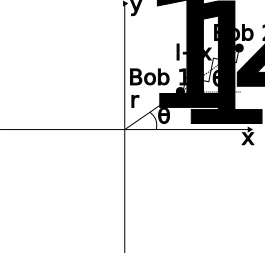
\includegraphics[width=300px]{Double pendulum second elastic.png}
	\caption{Diagram of a double pendulum wherein the second pendulum is elastic.}
\end{figure}

\subsection{Positions and velocities}
The Cartesian coordinates (and time derivatives thereof) of the first pendulum bob are
\begin{align*}
	x_1 &= r \cos{\theta_1} &\therefore \dot{x}_1 &= -r \dot{\theta}_1 \sin{\theta_1}\\
	y_1 &= r \sin{\theta_1} &\therefore \dot{y}_1 &= r \dot{\theta}_1 \cos{\theta_1}
\end{align*}

As for the second pendulum bob has the coordinates (and time derivatives thereof)
\begin{align*}
	x_2 &= x_1 + (l+z)\cos{\theta_2} & \therefore v_1^2 &= r^2 \dot{\theta}_1^2\\
	&= r \cos{\theta_1} + (l+z)\cos{\theta_2} &\therefore \dot{x}_2 &= -r \dot{\theta}_1 \sin{\theta_1} + \dot{z} \cos{\theta_2}-(l+z)\dot{\theta}_2 \sin{\theta_2}\\
	y_2 &= y_1 + (l+z)\sin{\theta_2} \\
	&= r\sin{\theta_1} + (l+z)\sin{\theta_2} &\therefore \dot{y}_2 &= r \dot{\theta}_1 \cos{\theta_1} + \dot{z} \sin{\theta_2}+(l+z)\dot{\theta}_2 \cos{\theta_2}.
\end{align*}

Hence the velocity of the first pendulum bob is
\begin{align*}
	\vec{v}_1 &= \begin{bmatrix}
		\dot{x}_1 \\
		\dot{y}_1
	\end{bmatrix} & \vec{v}_2 &= \begin{bmatrix}
		\dot{x}_2 \\
		\dot{y}_2
	\end{bmatrix} \\
	&= r\dot{\theta}_1\begin{bmatrix}
		-\sin{\theta_1} \\
		\cos{\theta_1}
	\end{bmatrix} & &= \begin{bmatrix}
		-r \dot{\theta}_1 \sin{\theta_1} + \dot{z} \cos{\theta_2}-(l+z)\dot{\theta}_2 \sin{\theta_2} \\
		r \dot{\theta}_1 \cos{\theta_1} + \dot{z} \sin{\theta_2}+(l+z)\dot{\theta}_2 \cos{\theta_2}
	\end{bmatrix}\\
	|\vec{v}_1| &= r|\dot{\theta}_1|.
\end{align*}
The second pendulum bob has the velocity
\begin{align*}
	|\vec{v}_2|^2 &= \left( -r \dot{\theta}_1 \sin{\theta_1} + \dot{z} \cos{\theta_2}-(l+z)\dot{\theta}_2 \sin{\theta_2}\right)^2 + \left(r \dot{\theta}_1 \cos{\theta_1} + \dot{z} \sin{\theta_2}+(l+z)\dot{\theta}_2 \cos{\theta_2}\right)^2 \\
	&= r^2 \dot{\theta}_1^2 \sin^2{\theta_1}+\dot{z}^2 \cos^2{\theta_2}+(l+z)^2 \dot{\theta}_2^2 \sin^2{\theta_2} - 2r \dot{\theta}_1 \dot{z}\sin{\theta_1}\cos{\theta_2} + 2r (l+z)\dot{\theta}_1 \dot{\theta}_2 \sin{\theta_1}\sin{\theta_2}\\
	&-2\dot{z}(l+z)\dot{\theta}_2 \cos{\theta_2}\sin{\theta_2}+r^2\dot{\theta}_1^2 \cos^2{\theta_1} + \dot{z}^2 \sin^2{\theta_2} + (l+z)^2 \dot{\theta}_2^2\cos^2{\theta_2} + 2r(l+z)\dot{\theta}_1\dot{\theta}_2\cos{\theta_1}\cos{\theta_2}\\
	&+2r\dot{z}\dot{\theta}_1 \cos{\theta_1}\sin{\theta_2}+2\dot{z}\dot{\theta}_2(l+z)\sin{\theta_2}\cos{\theta_2} \\
	&= r^2 \dot{\theta}_1^2 + \dot{z}^2 + (l+z)^2\dot{\theta}_2^2 + 2r\dot{\theta}_1 \dot{z} (\cos{\theta_1}\sin{\theta_2} - \sin{\theta_1}\cos{\theta_2}) + 2r(l+z)\dot{\theta}_1\dot{\theta}_2(\sin{\theta_1}\sin{\theta_2} + \cos{\theta_1}\cos{\theta_2})\\
	&+2\dot{z}\dot{\theta}_2(l+z)(\sin{\theta_2}\cos{\theta_2}-\sin{\theta_2}\cos{\theta_2})\\
	&= r^2 \dot{\theta}_1^2 + \dot{z}^2 + (l+z)^2\dot{\theta}_2^2 + 2r\dot{\theta}_1 \dot{z} \sin{(\theta_2-\theta_1)} + 2r(l+z)\dot{\theta}_1\dot{\theta}_2\cos{(\theta_2 - \theta_1)} \\
	|\vec{v}_2| &= \sqrt{r^2 \dot{\theta}_1^2 + \dot{z}^2 + (l+z)^2\dot{\theta}_2^2 + 2r\dot{\theta}_1 \dot{z} \sin{(\theta_2-\theta_1)} + 2r(l+z)\dot{\theta}_1\dot{\theta}_2\cos{(\theta_2 - \theta_1)}}.
\end{align*}
\subsection{Generalized basis vectors}
The generalized basis vectors for this system are given by
\begin{align*}
	\hat{e}_{1, \theta_1} &= \dfrac{\partial \vec{r}_1}{\partial \theta_1} & \hat{e}_{1, z} &= \dfrac{\partial \vec{r}_1}{\partial z} \\
	&= r\begin{bmatrix}
		-\sin{\theta_1} \\
		\cos{\theta_1}
	\end{bmatrix} & &= 0 \\
	 \hat{e}_{1, \theta_2} &= \dfrac{\partial \vec{r}_1}{\partial \theta_2} & \hat{e}_{2, \theta_1} &= \dfrac{\partial \vec{r}_2}{\partial \theta_1} \\
	 &=0 & &= r\begin{bmatrix}
	 	-\sin{\theta_1} \\
	 	\cos{\theta_1}
	 \end{bmatrix} \\
	\hat{e}_{2, \theta_2} &= \dfrac{\partial \vec{r}_2}{\partial \theta_2} & \hat{e}_{2, z} &=\dfrac{\partial \vec{r}_2}{\partial z}\\
	&= (l+z)\begin{bmatrix}
		-\sin{\theta_2} \\
		\cos{\theta_2}
	\end{bmatrix} & &= \begin{bmatrix}
	\cos{\theta_2}\\
	\sin{\theta_2}
	\end{bmatrix}.
\end{align*}

\subsection{Kinetic energy}
\begin{align*}
	T &= \dfrac{m_1}{2}|\vec{v}_1|^2 + \dfrac{m_2}{2}|\vec{v}_2|^2 \\
	&= \dfrac{m_1r^2 \dot{\theta}_1^2}{2} + \dfrac{m_2(r^2 \dot{\theta}_1^2 + \dot{z}^2 + (l+z)^2\dot{\theta}_2^2 + 2r\dot{\theta}_1 \dot{z} \sin{(\theta_2-\theta_1)} + 2r(l+z)\dot{\theta}_1\dot{\theta}_2\cos{(\theta_2 - \theta_1)})}{2}\\
	&= \dfrac{m_1+m_2}{2}r^2\dot{\theta}_1^2 + \dfrac{m_2(\dot{z}^2 + (l+z)^2\dot{\theta}_2^2 + 2r\dot{\theta}_1[ \dot{z} \sin{(\theta_2-\theta_1)} + (l+z)\dot{\theta}_2\cos{(\theta_2 - \theta_1)}])}{2}.
\end{align*}

\subsection{Potential energy}
\subsubsection{First bob}
For the first bob, the only potential energy is gravitational. 
\begin{align*}
	V_1 &= m_1gy_1 \\
	&= m_1 gr\sin{\theta_1}.
\end{align*}

\subsubsection{Second bob}
For the second bob, there is the spring potential energy and the gravitational potential energy to consider

\begin{align*}
	V_2 &= m_2gy_2 + \dfrac{kz^2}{2} \\
	&= m_2 g(r\sin{\theta_1} + (l+z)\sin{\theta_2}) + \dfrac{kz^2}{2}.
\end{align*}

\subsubsection{Total}
The total potential energy is therefore

\begin{align*}
	V &= V_1 + V_2 \\
	&= m_1 gr\sin{\theta_1} + m_2 g(r\sin{\theta_1} + (l+z)\sin{\theta_2}) + \dfrac{kz^2}{2}.
\end{align*}
\begin{landscape}
\subsection{Lagrangian}
\begin{align*}
	\lag &= T - V \\
	&= \dfrac{m_1+m_2}{2}r^2\dot{\theta}_1^2 + \dfrac{m_2(\dot{z}^2 + (l+z)^2\dot{\theta}_2^2 + 2r\dot{\theta}_1[ \dot{z} \sin{(\theta_2-\theta_1)} + (l+z)\dot{\theta}_2\cos{(\theta_2 - \theta_1)}])}{2} - m_1 gr\sin{\theta_1} \\
	&- m_2 g(r\sin{\theta_1} + (l+z)\sin{\theta_2}) - \dfrac{kz^2}{2}. \\
	&= \dfrac{m_1+m_2}{2}\left(r^2\dot{\theta}_1^2-2gr\sin{\theta_1}\right) + \dfrac{m_2}{2}\left(\dot{z}^2 + (l+z)^2\dot{\theta}_2^2 + 2r\dot{\theta}_1[ \dot{z} \sin{(\theta_2-\theta_1)} + (l+z)\dot{\theta}_2\cos{(\theta_2 - \theta_1)}]-2g(l+z)\sin{\theta_2}\right) - \dfrac{kz^2}{2}.
\end{align*}

\subsection{Euler-Lagrange equations}
\subsubsection{$\theta_1$}
\begin{align*}
	p_{\theta_1} &= \dfrac{\partial \lag}{\partial \dot{\theta}_1} \\
	&= (m_1+m_2)r^2 \dot{\theta}_1 + m_2r[ \dot{z} \sin{(\theta_2-\theta_1)} + (l+z)\dot{\theta}_2\cos{(\theta_2 - \theta_1)}] \\
	\dot{p}_{\theta_1} &= (m_1+m_2)r^2 \ddot{\theta}_1 +  m_2r[ \ddot{z} \sin{(\theta_2-\theta_1)} + \dot{z}(\dot{\theta}_2-\dot{\theta}_1)\cos{(\theta_2-\theta_1)}+ (l+z)\ddot{\theta}_2\cos{(\theta_2 - \theta_1)}- (l+z)\dot{\theta}_2(\dot{\theta}_2-\dot{\theta}_1)\sin{(\theta_2 - \theta_1)}+\dot{z}\dot{\theta}_2\cos{(\theta_2 - \theta_1)}]\\
	&= (m_1+m_2)r^2 \ddot{\theta}_1 +  m_2r[(\ddot{z} -(l+z)\dot{\theta}_2(\dot{\theta}_2-\dot{\theta}_1))\sin{(\theta_2 - \theta_1)}+(\dot{z}(2\dot{\theta}_2-\dot{\theta}_1)+(l+z)\ddot{\theta}_2)\cos{(\theta_2-\theta_1)}]
\end{align*}

Calculating the generalized force for $\theta_1$ (a term taken from \href{https://phys.libretexts.org/Bookshelves/Classical_Mechanics/Graduate_Classical_Mechanics_(Fowler)/04%3A_Hamilton's_Principle_and_Noether's_Theorem/4.05%3A_Generalized_Momenta_and_Forces}{Fowler's Graduate Classical Mechanics})
\begin{align*}
	 F_{\theta_1} &= \dfrac{\partial \lag}{\partial \theta_1} \\
	 &= m_2 r \dot{\theta}_1(\dot{z}\cos{(\theta_2-\theta_1)}\cdot -1 -(l+z)\dot{\theta}_2 \sin{(\theta_2-\theta_1)}\cdot -1) - m_1gr \cos{\theta_1} - m_2gr\cos{\theta_1} \\
	 &= m_2 r\dot{\theta}_1((l+z)\dot{\theta}_2 \sin{(\theta_2-\theta_1)}-\dot{z}\cos{(\theta_2-\theta_1)}) -(m_1+m_2)gr\cos{\theta_1}
\end{align*}

As for the generalized dissipative force, it is

\begin{align*}
	Q_{\theta_1} &= \sum_{j=1}^2 \vec{F}_{D,j} \cdot \hat{e}_{j, \theta_1}.
\end{align*}

Where $j$ refers to the particle (bob 1 or bob 2) under consideration. 

\begin{align*}
	\vec{F}_{D, 1} &= -(b_1+c_1|\vec{v}_1|)\vec{v}_1 \\
	&= -(b_1+c_1r|\dot{\theta}_1|)r\dot{\theta}_1 \begin{bmatrix}
		-\sin{\theta}_1 \\
		\cos{\theta}_1
	\end{bmatrix} \\
	\vec{F}_{D, 2} &= -(b_2+c_2|\vec{v}_2|)\vec{v}_2 \\
	&= -\left(b_2+c_2\sqrt{r^2 \dot{\theta}_1^2 + \dot{z}^2 + (l+z)^2\dot{\theta}_2^2 + 2r\dot{\theta}_1 \dot{z} \sin{(\theta_2-\theta_1)} + 2r(l+z)\dot{\theta}_1\dot{\theta}_2\cos{(\theta_2 - \theta_1)}}\right)\\
	&\begin{bmatrix}
		-r \dot{\theta}_1 \sin{\theta_1} + \dot{z} \cos{\theta_2}-(l+z)\dot{\theta}_2 \sin{\theta_2} \\
		r \dot{\theta}_1 \cos{\theta_1} + \dot{z} \sin{\theta_2}+(l+z)\dot{\theta}_2 \cos{\theta_2}
	\end{bmatrix}.
\end{align*}

Hence

\begin{align*}
	Q_{\theta_1} &= -(b_1+c_1r|\dot{\theta}_1|)r\dot{\theta}_1 \begin{bmatrix}
		-\sin{\theta}_1 \\
		\cos{\theta}_1
	\end{bmatrix} \cdot r\begin{bmatrix}
	-\sin{\theta_1} \\
	\cos{\theta_1}
	\end{bmatrix} -\left(b_2+c_2\sqrt{r^2 \dot{\theta}_1^2 + \dot{z}^2 + (l+z)^2\dot{\theta}_2^2 + 2r\dot{\theta}_1 \dot{z} \sin{(\theta_2-\theta_1)} + 2r(l+z)\dot{\theta}_1\dot{\theta}_2\cos{(\theta_2 - \theta_1)}}\right)\\
	&\begin{bmatrix}
	-r \dot{\theta}_1 \sin{\theta_1} + \dot{z} \cos{\theta_2}-(l+z)\dot{\theta}_2 \sin{\theta_2} \\
	r \dot{\theta}_1 \cos{\theta_1} + \dot{z} \sin{\theta_2}+(l+z)\dot{\theta}_2 \cos{\theta_2}
	\end{bmatrix} \cdot  r\begin{bmatrix}
	-\sin{\theta_1} \\
	\cos{\theta_1}
	\end{bmatrix} \\
	&= -(b_1+c_1r|\dot{\theta}_1|)r^2\dot{\theta}_1 -\left(b_2+c_2\sqrt{r^2 \dot{\theta}_1^2 + \dot{z}^2 + (l+z)^2\dot{\theta}_2^2 + 2r\dot{\theta}_1 \dot{z} \sin{(\theta_2-\theta_1)} + 2r(l+z)\dot{\theta}_1\dot{\theta}_2\cos{(\theta_2 - \theta_1)}}\right)\left(r^2\dot{\theta}_1\sin^2{\theta_1} - r\dot{z}\sin{\theta_1}\cos{\theta_2} + r(l+z)\dot{\theta}_2 \sin{\theta_1}\sin{\theta_2}\right.\\
	&\left.+r^2\dot{\theta}_1 \cos^2{\theta_1} + r\dot{z}\cos{\theta_1}\sin{\theta_2}+r(l+z)\dot{\theta}_2\cos{\theta_2}\cos{\theta_1}\right) \\
	&= -(b_1+c_1r|\dot{\theta}_1|)r^2\dot{\theta}_1 -\left(b_2+c_2\sqrt{r^2 \dot{\theta}_1^2 + \dot{z}^2 + (l+z)^2\dot{\theta}_2^2 + 2r\dot{\theta}_1 \dot{z} \sin{(\theta_2-\theta_1)} + 2r(l+z)\dot{\theta}_1\dot{\theta}_2\cos{(\theta_2 - \theta_1)}}\right)\left(r^2\dot{\theta}_1 + r\dot{z}\sin{(\theta_2-\theta_1)} + r(l+z)\dot{\theta}_2 \cos{(\theta_2-\theta_1)}\right).
\end{align*}

$Q_{\theta_1}$ is complicated and does not involve second time derivatives, so there is no point writing it out in full from here on. 

The left-hand side of \eq{ELD} is therefore

\begin{align*}
	&(m_1+m_2)r^2 \ddot{\theta}_1 +  m_2r[(\ddot{z} -(l+z)\dot{\theta}_2(\dot{\theta}_2-\dot{\theta}_1))\sin{(\theta_2 - \theta_1)}+(\dot{z}(2\dot{\theta}_2-\dot{\theta}_1)+(l+z)\ddot{\theta}_2)\cos{(\theta_2-\theta_1)}] \\
	& -\left(m_2 r\dot{\theta}_1((l+z)\dot{\theta}_2 \sin{(\theta_2-\theta_1)}-\dot{z}\cos{(\theta_2-\theta_1)}) -(m_1+m_2)gr\cos{\theta_1}\right)\\
	&= (m_1+m_2)r (r\ddot{\theta}_1+g\cos{\theta_1}) +  m_2r[(\ddot{z} -(l+z)\dot{\theta}_2^2)\sin{(\theta_2 - \theta_1)}+(2\dot{z}\dot{\theta}_2+(l+z)\ddot{\theta}_2)\cos{(\theta_2-\theta_1)}].
\end{align*}

Hence \eq{ELD} is

\begin{align*}
	(m_1+m_2)r (r\ddot{\theta}_1+g\cos{\theta_1}) +  m_2r[(\ddot{z} -(l+z)\dot{\theta}_2^2)\sin{(\theta_2 - \theta_1)}+(2\dot{z}\dot{\theta}_2+(l+z)\ddot{\theta}_2)\cos{(\theta_2-\theta_1)}] &= Q_{\theta_1}.
\end{align*}

Dividing both sides by $(m_1+m_2)r^2$ gives

\begin{align*}
	\ddot{\theta}_1 + \dfrac{g}{r}\cos{\theta_1} + \dfrac{m_2}{(m_1+m_2)r}\left[(\ddot{z} -(l+z)\dot{\theta}_2^2)\sin{(\theta_2 - \theta_1)}+(2\dot{z}\dot{\theta}_2+(l+z)\ddot{\theta}_2)\cos{(\theta_2-\theta_1)}\right] &= \dfrac{Q_{\theta_1}}{(m_1+m_2)r^2}.
\end{align*}

Moving everything but the $\ddot{\theta}_1$ to the RHS yields

\begin{align}
	\ddot{\theta}_1 &= \dfrac{Q_{\theta_1}}{(m_1+m_2)r^2} - \dfrac{g}{r}\cos{\theta_1} - \dfrac{m_2}{(m_1+m_2)r}\left[(\ddot{z} -(l+z)\dot{\theta}_2^2)\sin{(\theta_2 - \theta_1)}+(2\dot{z}\dot{\theta}_2+(l+z)\ddot{\theta}_2)\cos{(\theta_2-\theta_1)}\right]. \label{d2theta1}
\end{align}

\subsubsection{$\theta_2$}
Hence

\begin{align*}
	p_{\theta_2} &= \dfrac{\partial \lag}{\partial \dot{\theta}_2} \\
	&= m_2(l+z)\left[(l+z)\dot{\theta}_2 + r\dot{\theta}_1\cos{(\theta_2-\theta_1)}\right] \\
	\dot{p}_{\theta_2} &= m_2\dot{z}\left[(l+z)\dot{\theta}_2 + r\dot{\theta}_1\cos{(\theta_2-\theta_1)}\right] + m_2(l+z)\left[\dot{z}\dot{\theta}_2 + (l+z)\ddot{\theta}_2 + r\ddot{\theta}_1\cos{(\theta_2-\theta_1)} - r\dot{\theta}_1(\dot{\theta}_2-\dot{\theta}_1)\sin{(\theta_2-\theta_1)}\right]\\
	&= m_2 \left[r\dot{\theta}_1\dot{z}\cos{(\theta_2-\theta_1)} + (l+z)\left(2\dot{z}\dot{\theta}_2 + (l+z)\ddot{\theta}_2+ r\ddot{\theta}_1\cos{(\theta_2-\theta_1)} - r\dot{\theta}_1(\dot{\theta}_2-\dot{\theta}_1)\sin{(\theta_2-\theta_1)}\right)\right]\\
	F_{\theta_2} &= \dfrac{\partial \lag}{\partial \theta_2} \\
	&= m_2 \left[r\dot{\theta}_1 \left(\dot{z}\cos{(\theta_2-\theta_1)}-(l+z)\dot{\theta}_2\sin{(\theta_2-\theta_1)}\right)-g(l+z)\cos{\theta_2}\right]\\
	Q_{\theta_2} &= \vec{F}_{D,1} \cdot \hat{e}_{1,\theta_2} + \vec{F}_{D,2} \cdot \hat{e}_{2,\theta_2} \\
	&= -(b_1+c_1r|\dot{\theta}_1|)r\dot{\theta}_1 \begin{bmatrix}
		-\sin{\theta}_1 \\
		\cos{\theta}_1
	\end{bmatrix} \cdot \vec{0} - \left(b_2+c_2\sqrt{r^2 \dot{\theta}_1^2 + \dot{z}^2 + (l+z)^2\dot{\theta}_2^2 + 2r\dot{\theta}_1 \dot{z} \sin{(\theta_2-\theta_1)} + 2r(l+z)\dot{\theta}_1\dot{\theta}_2\cos{(\theta_2 - \theta_1)}}\right)\\
	&\begin{bmatrix}
	-r \dot{\theta}_1 \sin{\theta_1} + \dot{z} \cos{\theta_2}-(l+z)\dot{\theta}_2 \sin{\theta_2} \\
	r \dot{\theta}_1 \cos{\theta_1} + \dot{z} \sin{\theta_2}+(l+z)\dot{\theta}_2 \cos{\theta_2}
	\end{bmatrix}\cdot (l+z)\begin{bmatrix}
	-\sin{\theta_2} \\
	\cos{\theta_2}
	\end{bmatrix} \\
	&= - \left(b_2+c_2\sqrt{r^2 \dot{\theta}_1^2 + \dot{z}^2 + (l+z)^2\dot{\theta}_2^2 + 2r\dot{\theta}_1 \dot{z} \sin{(\theta_2-\theta_1)} + 2r(l+z)\dot{\theta}_1\dot{\theta}_2\cos{(\theta_2 - \theta_1)}}\right)(l+z)\left[r\dot{\theta}_1 \sin{\theta_1}\sin{\theta_2} - \dot{z}\cos{\theta_2}\sin{\theta_2} + (l+z)\dot{\theta}_2\sin^2{\theta_2} \right.\\
	&\left.+ r\dot{\theta}_1 \cos{\theta_1}\cos{\theta_2} + \dot{z}\sin{\theta_2}\cos{\theta_2} + (l+z)\dot{\theta}_2\cos^2{\theta_2}\right] \\
	&= - \left(b_2+c_2\sqrt{r^2 \dot{\theta}_1^2 + \dot{z}^2 + (l+z)^2\dot{\theta}_2^2 + 2r\dot{\theta}_1 \dot{z} \sin{(\theta_2-\theta_1)} + 2r(l+z)\dot{\theta}_1\dot{\theta}_2\cos{(\theta_2 - \theta_1)}}\right)(l+z)\left[r\dot{\theta}_1 \cos{(\theta_2-\theta_1)} + (l+z)\dot{\theta}_2 \right].
\end{align*}

So \eq{ELD} becomes

\begin{align*}
	&m_2 \left[r\dot{\theta}_1\dot{z}\cos{(\theta_2-\theta_1)} + (l+z)\left(2\dot{z}\dot{\theta}_2 + (l+z)\ddot{\theta}_2+ r\ddot{\theta}_1\cos{(\theta_2-\theta_1)} - r\dot{\theta}_1(\dot{\theta}_2-\dot{\theta}_1)\sin{(\theta_2-\theta_1)}\right)\right] - m_2 \left[r\dot{\theta}_1\right.\\ &\left.\left(\dot{z}\cos{(\theta_2-\theta_1)}-(l+z)\dot{\theta}_2\sin{(\theta_2-\theta_1)}\right)-g(l+z)\cos{\theta_2}\right] = Q_{\theta_2}\\
	&m_2(l+z)\left(2\dot{z}\dot{\theta}_2 + (l+z)\ddot{\theta}_2+ r\ddot{\theta}_1\cos{(\theta_2-\theta_1)} + r\dot{\theta}_1^2\sin{(\theta_2-\theta_1)}+g\cos{\theta_2}\right) = Q_{\theta_2}\\
\end{align*}

Dividing by $m_2 (l+z)^2$ yields

\begin{align*}
	\ddot{\theta}_2 + \dfrac{1}{l+z}\left[2\dot{z}\dot{\theta}_2 + r\ddot{\theta}_1 \cos{(\theta_2-\theta_1)} + r\dot{\theta}_1^2\sin{(\theta_2-\theta_1)} + g\cos{\theta}_2\right] &= \dfrac{Q_{\theta_2}}{m_2(l+z)^2}.
\end{align*}

Moving everything but $\ddot{\theta}_2$ to the right-hand side yields

\begin{align}
	\ddot{\theta}_2 &= -\dfrac{1}{l+z}\left[2\dot{z}\dot{\theta}_2 + r\ddot{\theta}_1 \cos{(\theta_2-\theta_1)} + r\dot{\theta}_1^2\sin{(\theta_2-\theta_1)} + g\cos{\theta}_2\right] + \dfrac{Q_{\theta_2}}{m_2(l+z)^2}. \label{d2theta2}
\end{align}

\subsubsection{$z$}
\begin{align*}
	p_z &= \dfrac{\partial \lag}{\partial \dot{z}} \\
	&= m_2\left(\dot{z} + r\dot{\theta}_1 \sin{(\theta_2-\theta_1)}\right) \\
	\dot{p}_z &= m_2 \left(\ddot{z} + r\ddot{\theta}_1 \sin{(\theta_2-\theta_1)} + r\dot{\theta}_1(\dot{\theta}_2-\dot{\theta}_1)\cos{(\theta_2-\theta_1)}\right) \\
	F_z &= \dfrac{\partial \lag}{\partial z} \\
	&= m_2 \left((l+z)\dot{\theta}_2^2 + r\dot{\theta}_1\dot{\theta}_2 \cos{(\theta_2-\theta_1)}-g\sin{\theta_2}\right) -kz\\
	Q_z &= \vec{F}_{D,1} \cdot \hat{e}_{1,z} + \vec{F}_{D,2} \cdot \hat{e}_{2,z} \\
	&= -(b_1+c_1r|\dot{\theta}_1|)r\dot{\theta}_1 \begin{bmatrix}
		-\sin{\theta}_1 \\
		\cos{\theta}_1
	\end{bmatrix} \cdot \vec{0}-\left(b_2+c_2\sqrt{r^2 \dot{\theta}_1^2 + \dot{z}^2 + (l+z)^2\dot{\theta}_2^2 + 2r\dot{\theta}_1 \dot{z} \sin{(\theta_2-\theta_1)} + 2r(l+z)\dot{\theta}_1\dot{\theta}_2\cos{(\theta_2 - \theta_1)}}\right)\\
	&\begin{bmatrix}
	-r \dot{\theta}_1 \sin{\theta_1} + \dot{z} \cos{\theta_2}-(l+z)\dot{\theta}_2 \sin{\theta_2} \\
	r \dot{\theta}_1 \cos{\theta_1} + \dot{z} \sin{\theta_2}+(l+z)\dot{\theta}_2 \cos{\theta_2}
	\end{bmatrix} \cdot \begin{bmatrix}
	\cos{\theta_2}\\
	\sin{\theta_2}
	\end{bmatrix} \\
	&= -\left(b_2+c_2\sqrt{r^2 \dot{\theta}_1^2 + \dot{z}^2 + (l+z)^2\dot{\theta}_2^2 + 2r\dot{\theta}_1 \dot{z} \sin{(\theta_2-\theta_1)} + 2r(l+z)\dot{\theta}_1\dot{\theta}_2\cos{(\theta_2 - \theta_1)}}\right)\left[-r\dot{\theta}_1 \sin{\theta_1}\cos{\theta_2} \right.\\
	&\left.+ \dot{z}\cos^2{\theta_2} -(l+z)\dot{\theta}_2 \sin{\theta_2}\cos{\theta_2} + r\dot{\theta}_1\cos{\theta_1}\sin{\theta_2} + \dot{z}\sin^2{\theta_2} + (l+z)\dot{\theta}_2 \cos{\theta_2}\sin{\theta_2}\right] \\
	&= -\left(b_2+c_2\sqrt{r^2 \dot{\theta}_1^2 + \dot{z}^2 + (l+z)^2\dot{\theta}_2^2 + 2r\dot{\theta}_1 \dot{z} \sin{(\theta_2-\theta_1)} + 2r(l+z)\dot{\theta}_1\dot{\theta}_2\cos{(\theta_2 - \theta_1)}}\right)\left[r\dot{\theta}_1\sin{(\theta_2-\theta_1)} + \dot{z}\right].
\end{align*}

Hence \eq{ELD} becomes

\begin{align*}
	m_2 \left(\ddot{z} + r\ddot{\theta}_1 \sin{(\theta_2-\theta_1)} + r\dot{\theta}_1(\dot{\theta}_2-\dot{\theta}_1)\cos{(\theta_2-\theta_1)}\right) - \left(m_2 \left((l+z)\dot{\theta}_2^2 + r\dot{\theta}_1\dot{\theta}_2 \cos{(\theta_2-\theta_1)}-g\sin{\theta_2}\right) -kz\right) &= Q_z \\
	m_2\left[\ddot{z} + r\ddot{\theta}_1 \sin{(\theta_2-\theta_1)} - r\dot{\theta}_1^2\cos{(\theta_2-\theta_1)} - (l+z)\dot{\theta}_2^2+g\sin{\theta_2}\right]+kz &= Q_z.
\end{align*}

Dividing by $m_2$ yields

\begin{align*}
	\ddot{z} + r\ddot{\theta}_1 \sin{(\theta_2-\theta_1)} - r\dot{\theta}_1^2\cos{(\theta_2-\theta_1)} - (l+z)\dot{\theta}_2^2+g\sin{\theta_2} + k'z &= \dfrac{Q_z}{m_2}
\end{align*}

where $k'=\dfrac{k}{m_2}$. Moving everything but the $\ddot{z}$ term to the right-hand side

\begin{align}
	\ddot{z} &= -r\ddot{\theta}_1 \sin{(\theta_2-\theta_1)} + r\dot{\theta}_1^2\cos{(\theta_2-\theta_1)} + (l+z)\dot{\theta}_2^2-g\sin{\theta_2} - k'z + \dfrac{Q_z}{m_2}. \label{d2z}
\end{align}

Let us substitute \eq{d2z} into \eq{d2theta1}

\begin{align*}
	\ddot{\theta}_1 &= \dfrac{Q_{\theta_1}}{(m_1+m_2)r^2} - \dfrac{g}{r}\cos{\theta_1} - \dfrac{m_2}{(m_1+m_2)r}\left[(-r\ddot{\theta}_1 \sin{(\theta_2-\theta_1)} + r\dot{\theta}_1^2\cos{(\theta_2-\theta_1)} + (l+z)\dot{\theta}_2^2-g\sin{\theta_2} - k'z + \dfrac{Q_z}{m_2} -(l+z)\dot{\theta}_2^2)\sin{(\theta_2 - \theta_1)}\right.\\
	&\left.+(2\dot{z}\dot{\theta}_2+(l+z)\ddot{\theta}_2)\cos{(\theta_2-\theta_1)}\right]\\
	\ddot{\theta}_1 \left(1-\dfrac{m_2\sin^2{(\theta_2-\theta_1)}}{m_1+m_2}\right)&= \dfrac{Q_{\theta_1}}{(m_1+m_2)r^2} - \dfrac{g}{r}\cos{\theta_1} - \dfrac{m_2}{(m_1+m_2)r}\left[\left(r\dot{\theta}_1^2\cos{(\theta_2-\theta_1)}-g\sin{\theta_2} - k'z + \dfrac{Q_z}{m_2}\right)\sin{(\theta_2 - \theta_1)}+(2\dot{z}\dot{\theta}_2+(l+z)\ddot{\theta}_2)\cos{(\theta_2-\theta_1)}\right]
\end{align*}
\begin{align*}
	\dfrac{\ddot{\theta}_1}{m_1+m_2}(m_1+m_2 - m_2\sin^2{(\theta_2-\theta_1)}) &= \dfrac{Q_{\theta_1}}{(m_1+m_2)r^2} - \dfrac{g}{r}\cos{\theta_1} - \dfrac{m_2}{(m_1+m_2)r}\left[\left(r\dot{\theta}_1^2\cos{(\theta_2-\theta_1)}-g\sin{\theta_2} - k'z + \dfrac{Q_z}{m_2}\right)\sin{(\theta_2 - \theta_1)}\right.\\
	&\left.+(2\dot{z}\dot{\theta}_2+(l+z)\ddot{\theta}_2)\cos{(\theta_2-\theta_1)}\right] \\
	\dfrac{\ddot{\theta}_1}{m_1+m_2}(m_1+m_2\cos^2{(\theta_2-\theta_1)}) &= \dfrac{Q_{\theta_1}}{(m_1+m_2)r^2} - \dfrac{g}{r}\cos{\theta_1} - \dfrac{m_2}{(m_1+m_2)r}\left[\left(r\dot{\theta}_1^2\cos{(\theta_2-\theta_1)}-g\sin{\theta_2} - k'z + \dfrac{Q_z}{m_2}\right)\sin{(\theta_2 - \theta_1)}\right.\\
	&\left.+(2\dot{z}\dot{\theta}_2+(l+z)\ddot{\theta}_2)\cos{(\theta_2-\theta_1)}\right]
\end{align*}

\begin{align}
	\therefore \ddot{\theta}_1 &= \dfrac{1}{(m_1+m_2\cos^2{(\theta_2-\theta_1)})r^2}\left[Q_{\theta_1} - g(m_1+m_2)r\cos{\theta_1} + r(kz-Q_z)\sin{(\theta_2-\theta_1)} - m_2r\left((r\dot{\theta}_1^2\cos{(\theta_2-\theta_1)}-g\sin{\theta_2})\sin{(\theta_2 - \theta_1)}\right.\right.\nonumber\\
	&\left.\left.+(2\dot{z}\dot{\theta}_2+(l+z)\ddot{\theta}_2)\cos{(\theta_2-\theta_1)}\right)\right]\label{d2theta1wd2theta2}
\end{align}

We will substitute \eq{d2theta1wd2theta2} into \eq{d2theta2}. Let us first calculate what $\dfrac{-r\ddot{\theta}_1 \cos{(\theta_2-\theta_1)}}{l+z}$ equals

\begin{align*}
	\dfrac{-r\ddot{\theta}_1 \cos{(\theta_2-\theta_1)}}{l+z} &= \dfrac{m_2\ddot{\theta}_2\cos^2{(\theta_2-\theta_1)}}{m_1+m_2\cos^2{(\theta_2-\theta_1)}} + \dfrac{\cos{(\theta_2-\theta_1)}}{(m_1+m_2\cos^2{(\theta_2-\theta_1)})r(l+z)}\left[m_2r\left((r\dot{\theta}_1^2\cos{(\theta_2-\theta_1)}-g\sin{\theta_2})\sin{(\theta_2 - \theta_1)}+2\dot{z}\dot{\theta}_2\cos{(\theta_2-\theta_1)}\right)-Q_{\theta_1}\right.\\
	&\left.-r(kz-Q_z)\sin{(\theta_2-\theta_1)}+g(m_1+m_2)r\cos{\theta_1}\right] \\
	&= \dfrac{m_2\ddot{\theta}_2\cos^2{(\theta_2-\theta_1)}}{m_1+m_2\cos^2{(\theta_2-\theta_1)}} + \dfrac{m_2r\dot{\theta}_1^2 \cos^2{(\theta_2-\theta_1)}\sin{(\theta_2-\theta_1)}}{(m_1+m_2\cos^2{(\theta_2-\theta_1)})(l+z)} + \dfrac{\cos{(\theta_2-\theta_1)}}{(m_1+m_2\cos^2{(\theta_2-\theta_1)})r(l+z)}\left[m_2r\left(-g\sin{\theta_2}\sin{(\theta_2 - \theta_1)}\right.\right.\\
	&\left.\left.+2\dot{z}\dot{\theta}_2\cos{(\theta_2-\theta_1)}\right)-Q_{\theta_1}-r(kz-Q_z)\sin{(\theta_2-\theta_1)}+g(m_1+m_2)r\cos{\theta_1}\right] \\
	&= \dfrac{m_2\ddot{\theta}_2\cos^2{(\theta_2-\theta_1)}}{m_1+m_2\cos^2{(\theta_2-\theta_1)}} + \dfrac{r\dot{\theta}_1^2\sin{(\theta_2-\theta_1)}}{l+z}\left[1-\dfrac{m_1}{m_1+m_2\cos^2{(\theta_2-\theta_1)}}\right] + \dfrac{\cos{(\theta_2-\theta_1)}}{(m_1+m_2\cos^2{(\theta_2-\theta_1)})r(l+z)}\left[m_2r\right.\\
	&\left.\left(-g\sin{\theta_2}\sin{(\theta_2 - \theta_1)}+2\dot{z}\dot{\theta}_2\cos{(\theta_2-\theta_1)}\right)-Q_{\theta_1}-r(kz-Q_z)\sin{(\theta_2-\theta_1)}+g(m_1+m_2)r\cos{\theta_1}\right].
\end{align*}

Hence 
\begin{align*}
	-\dfrac{r\ddot{\theta}_1 \cos{(\theta_2-\theta_1)}+r\dot{\theta}_1^2\sin{(\theta_2-\theta_1)}}{l+z} &= \dfrac{m_2\ddot{\theta}_2\cos^2{(\theta_2-\theta_1)}}{m_1+m_2\cos^2{(\theta_2-\theta_1)}} - \dfrac{m_1r\dot{\theta}_1^2\sin{(\theta_2-\theta_1)}}{(l+z)(m_1+m_2\cos^2{(\theta_2-\theta_1)})} + \dfrac{2m_2\cos^2{(\theta_2-\theta_1)}\dot{z}\dot{\theta}_2}{(m_1+m_2\cos^2{(\theta_2-\theta_1)})(l+z)}\\
	&- \dfrac{\cos{(\theta_2-\theta_1)}}{(m_1+m_2\cos^2{(\theta_2-\theta_1)})r(l+z)}\left[m_2gr\sin{\theta_2}\sin{(\theta_2 - \theta_1)}+Q_{\theta_1}+r(kz-Q_z)\sin{(\theta_2-\theta_1)}-g(m_1+m_2)r\cos{\theta_1}\right] \\
	&= \dfrac{m_2\ddot{\theta}_2\cos^2{(\theta_2-\theta_1)}}{m_1+m_2\cos^2{(\theta_2-\theta_1)}} - \dfrac{m_1r\dot{\theta}_1^2\sin{(\theta_2-\theta_1)}}{(l+z)(m_1+m_2\cos^2{(\theta_2-\theta_1)})} + \dfrac{2\dot{z}\dot{\theta}_2}{l+z}\left[1-\dfrac{m_1}{m_1+m_2\cos^2{(\theta_2-\theta_1)}}\right]\\
	&- \dfrac{\cos{(\theta_2-\theta_1)}}{(m_1+m_2\cos^2{(\theta_2-\theta_1)})r(l+z)}\left[m_2gr\sin{\theta_2}\sin{(\theta_2 - \theta_1)}+Q_{\theta_1}+r(kz-Q_z)\sin{(\theta_2-\theta_1)}-g(m_1+m_2)r\cos{\theta_1}\right]
\end{align*}

Adding in the $-\dfrac{2\dot{z}\dot{\theta}_2}{l+z}$ term of \eq{d2theta2} yields

\begin{align*}
	-\dfrac{2\dot{z}\dot{\theta}_2 + r\ddot{\theta}_1 \cos{(\theta_2-\theta_1)}+r\dot{\theta}_1^2\sin{(\theta_2-\theta_1)}}{l+z} &= \dfrac{m_2\ddot{\theta}_2\cos^2{(\theta_2-\theta_1)}}{m_1+m_2\cos^2{(\theta_2-\theta_1)}} - \dfrac{m_1(r\dot{\theta}_1^2\sin{(\theta_2-\theta_1)}+2\dot{z}\dot{\theta}_2)}{(l+z)(m_1+m_2\cos^2{(\theta_2-\theta_1)})}\\
	&- \dfrac{\cos{(\theta_2-\theta_1)}}{(m_1+m_2\cos^2{(\theta_2-\theta_1)})r(l+z)}\left[m_2gr\sin{\theta_2}\sin{(\theta_2 - \theta_1)}+Q_{\theta_1}+r(kz-Q_z)\sin{(\theta_2-\theta_1)}-g(m_1+m_2)r\cos{\theta_1}\right]
\end{align*}

Hence

\begin{align*}
	\ddot{\theta}_2 &= -\dfrac{g\cos{\theta_2}}{l+z} + \dfrac{m_2\ddot{\theta}_2\cos^2{(\theta_2-\theta_1)}}{m_1+m_2\cos^2{(\theta_2-\theta_1)}} - \dfrac{m_1(r\dot{\theta}_1^2\sin{(\theta_2-\theta_1)}+2\dot{z}\dot{\theta}_2)}{(l+z)(m_1+m_2\cos^2{(\theta_2-\theta_1)})} + \dfrac{Q_{\theta_2}}{m_2(l+z)^2}\\
	&- \dfrac{\cos{(\theta_2-\theta_1)}}{(m_1+m_2\cos^2{(\theta_2-\theta_1)})r(l+z)}\left[m_2gr\sin{\theta_2}\sin{(\theta_2 - \theta_1)}+Q_{\theta_1}+r(kz-Q_z)\sin{(\theta_2-\theta_1)}-g(m_1+m_2)r\cos{\theta_1}\right]
\end{align*}

Moving the $\ddot{\theta}_2$ term on the RHS to the LHS

\begin{align*}
	\ddot{\theta}_2 \left(1-\dfrac{m_2\cos^2{(\theta_2-\theta_1)}}{m_1+m_2\cos^2{(\theta_2-\theta_1)}}\right) &= -\dfrac{g\cos{\theta_2}}{l+z} - \dfrac{m_1(r\dot{\theta}_1^2\sin{(\theta_2-\theta_1)}+2\dot{z}\dot{\theta}_2)}{(l+z)(m_1+m_2\cos^2{(\theta_2-\theta_1)})} + \dfrac{Q_{\theta_2}}{m_2(l+z)^2}\\
	&- \dfrac{\cos{(\theta_2-\theta_1)}}{(m_1+m_2\cos^2{(\theta_2-\theta_1)})r(l+z)}\left[m_2gr\sin{\theta_2}\sin{(\theta_2 - \theta_1)}+Q_{\theta_1}+r(kz-Q_z)\sin{(\theta_2-\theta_1)}-g(m_1+m_2)r\cos{\theta_1}\right] \\
	\dfrac{m_1\ddot{\theta}_2}{m_1+m_2\cos^2{(\theta_2-\theta_1)}} &= -\dfrac{g\cos{\theta_2}}{l+z} - \dfrac{m_1(r\dot{\theta}_1^2\sin{(\theta_2-\theta_1)}+2\dot{z}\dot{\theta}_2)}{(l+z)(m_1+m_2\cos^2{(\theta_2-\theta_1)})} + \dfrac{Q_{\theta_2}}{m_2(l+z)^2}\\
	&- \dfrac{\cos{(\theta_2-\theta_1)}}{(m_1+m_2\cos^2{(\theta_2-\theta_1)})r(l+z)}\left[m_2gr\sin{\theta_2}\sin{(\theta_2 - \theta_1)}+Q_{\theta_1}+r(kz-Q_z)\sin{(\theta_2-\theta_1)}-g(m_1+m_2)r\cos{\theta_1}\right]\\
	\ddot{\theta}_2 &= -\dfrac{m_1+m_2\cos^2{(\theta_2-\theta_1)}}{m_1}\left[\dfrac{Q_{\theta_2}}{m_2(l+z)^2} - \dfrac{g\cos{\theta_2}}{l+z}\right] - \dfrac{r\dot{\theta}_1^2\sin{(\theta_2-\theta_1)}+2\dot{z}\dot{\theta}_2}{l+z} \\
	&- \dfrac{\cos{(\theta_2-\theta_1)}}{m_1r(l+z)}\left[m_2gr\sin{\theta_2}\sin{(\theta_2 - \theta_1)}+Q_{\theta_1}+r(kz-Q_z)\sin{(\theta_2-\theta_1)}-g(m_1+m_2)r\cos{\theta_1}\right]
\end{align*}
\end{landscape}

\section{Double elastic pendulum}
\begin{figure}[H]
	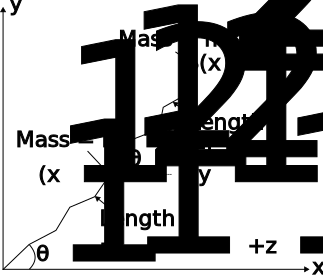
\includegraphics[width=\textwidth]{Double elastic pendulum.png}
	\caption{Diagram showing the double elastic pendulum.}
\end{figure}

As can be seen, we have four degrees of freedom in this system. The angles the two pendulums make with the positive $x$-axis --- $\theta_1$ and $\theta_2$, respectively --- are among our degrees of freedom. We will also need degrees of freedom corresponding to the lengths of the pendulum rods. These degrees of freedom could either be the extent to which they are extended beyond their rest length or their total length. For the sake of simplicity, we will opt to use their total lengths --- $r_1$ and $r_2$, respectively. Hence

\begin{align*}
	x_1 &= r_1 \cos{\theta_1} & \dot{x}_1 &= \dot{r}_1 \cos{\theta_1} - r_1 \dot{\theta}_1 \sin{\theta_1}\\
	y_1 &= r_1 \sin{\theta_1} & \dot{y}_1 &= \dot{r}_1\sin{\theta_1} + r_1\dot{\theta}_1 \cos{\theta_1} \\
	x_2 &= x_1 + r_2\cos{\theta_2} & \dot{x}_2 &= \dot{x}_1 + \dot{r}_2\cos{\theta_2} - r_2\dot{\theta}_2 \sin{\theta_2} \\
	y_2 &= y_1 + r_2\sin{\theta_2} & \dot{y}_2 &= \dot{y}_1 + \dot{r}_2\sin{\theta_2} + r_2\dot{\theta}_2 \cos{\theta_2}.
\end{align*}

This means that the velocity of the first pendulum bob is

\begin{align*}
	\vec{v}_1 &= \begin{bmatrix}
		\dot{x}_1 \\
		\dot{y}_1
	\end{bmatrix} \\
	&= \begin{bmatrix}
		\dot{r}_1 \cos{\theta_1} - r_1 \dot{\theta}_1 \sin{\theta_1} \\
		\dot{r}_1\sin{\theta_1} + r_1\dot{\theta}_1 \cos{\theta_1}
	\end{bmatrix} \\
	\therefore |\vec{v}_1|^2 &= \dot{r}_1^2 + r_1^2 \dot{\theta}_1^2. 
\end{align*}

As for the velocity of the second pendulum bob, it is
\begin{align*}
	\vec{v}_2 &= \begin{bmatrix}
		\dot{r}_1 \cos{\theta_1} - r_1 \dot{\theta}_1 \sin{\theta_1} + \dot{r}_2\cos{\theta_2} - r_2\dot{\theta}_2 \sin{\theta_2} \\
		\dot{r}_1\sin{\theta_1} + r_1\dot{\theta}_1 \cos{\theta_1} + \dot{r}_2\sin{\theta_2} + r_2\dot{\theta}_2 \cos{\theta_2}
	\end{bmatrix}
\end{align*}

\begin{landscape}
Let $\Delta = \theta_2-\theta_1$, then square of the velocity is

\begin{align*}
	|\vec{v}_2|^2 &= \dot{r}_1^2 \cos^2{\theta_1} + r_1^2 \dot{\theta}_1^2\sin^2{\theta_1} + \dot{r}_2^2\cos^2{\theta_2} + r_2^2\dot{\theta}_2^2\sin^2{\theta_2} -2r_1\dot{r}_1\dot{\theta}_1 \cos{\theta}_1\sin{\theta_1} + 2\dot{r}_1\dot{r}_2\cos{\theta_1}\cos{\theta_2} - 2\dot{r}_1r_2\dot{\theta}_2\cos{\theta_1}\sin{\theta_2} - 2r_1\dot{r}_2 \dot{\theta}_1 \sin{\theta_1}\cos{\theta_2} + 2r_1r_2 \dot{\theta}_1\dot{\theta}_2\sin{\theta_1}\sin{\theta_2}\\
	&-2\dot{r}_2r_2\dot{\theta}_2\cos{\theta_2}\sin{\theta_2} + \dot{r}_1^2\sin^2{\theta_1} + r_1^2\dot{\theta}_1^2\cos^2{\theta_1} + \dot{r}_2^2\sin^2{\theta_2} + r_2^2\dot{\theta}_2^2\cos^2{\theta_2} + 2r_1\dot{r}_1\dot{\theta}_1\sin{\theta_1}\cos{\theta_1} + 2\dot{r}_1\dot{r}_2\sin{\theta_1}\sin{\theta_2} + 2\dot{r}_1r_2\dot{\theta}_2\sin{\theta_1}\cos{\theta_2} + 2r_1\dot{r}_2\dot{\theta}_1 \cos{\theta_1}\sin{\theta_2}\\
	&+2r_1r_2\dot{\theta}_1\dot{\theta}_2\cos{\theta_1}\cos{\theta_2} + 2r_2\dot{r}_2\dot{\theta}_2\sin{\theta_2}\cos{\theta_2} \\
	&= \dot{r}_1^2 + r_1^2 \dot{\theta}_1^2 + \dot{r}_2^2 + r_2^2\dot{\theta}_2^2 + 2r_1\dot{r}_1\dot{\theta}_1(-\cos{\theta_1}\sin{\theta_1} + \cos{\theta_1}\sin{\theta_1}) + 2\dot{r}_1\dot{r}_2(\cos{\theta_1}\cos{\theta_2}+\sin{\theta_1}\sin{\theta_2})+2\dot{r}_1r_2\dot{\theta}_2(-\cos{\theta_1}\sin{\theta_2} + \sin{\theta_1}\cos{\theta_2}) \\
	&+ 2r_1\dot{r}_2\dot{\theta}_1(-\sin{\theta_1}\cos{\theta_2}+\cos{\theta_1}\sin{\theta_2}) + 2r_1r_2\dot{\theta}_1\dot{\theta}_2(\sin{\theta_1}\sin{\theta_2} + \cos{\theta_1}\cos{\theta_2}) + 2r_2\dot{r}_2\dot{\theta}_2 (-\cos{\theta_2}\sin{\theta_2} + \sin{\theta_2}\cos{\theta_2}) \\
	&= \dot{r}_1^2 + r_1^2 \dot{\theta}_1^2 + \dot{r}_2^2 + r_2^2\dot{\theta}_2^2 + 2\dot{r}_1\dot{r}_2 \cos{(\theta_2-\theta_1)} - 2\dot{r}_1r_2\dot{\theta_2}\sin{(\theta_2-\theta_1)} + 2r_1\dot{r}_2 \dot{\theta}_1 \sin{(\theta_2-\theta_1)} + 2r_1r_2\dot{\theta}_1\dot{\theta}_2\cos{(\theta_2-\theta_1)} \\
	&= \dot{r}_1^2 + r_1^2 \dot{\theta}_1^2 + \dot{r}_2^2 + r_2^2\dot{\theta}_2^2 + 2\dot{r}_1\dot{r}_2 \cos{\Delta} - 2\dot{r}_1r_2\dot{\theta_2}\sin{\Delta} + 2r_1\dot{r}_2 \dot{\theta}_1 \sin{\Delta} + 2r_1r_2\dot{\theta}_1\dot{\theta}_2\cos{\Delta} \\
	&= \dot{r}_1^2 + r_1^2 \dot{\theta}_1^2 + \dot{r}_2^2 + r_2^2\dot{\theta}_2^2 + 2\cos{\Delta}(\dot{r}_1\dot{r}_2 + r_1r_2\dot{\theta}_1\dot{\theta}_2) + 2\sin{\Delta}(r_1\dot{r}_2\dot{\theta}_1-\dot{r}_1r_2\dot{\theta}_2).
\end{align*}

Let us define $|\Delta \vec{v}_{21}|^2 = |\vec{v}_2|^2 - |\vec{v}_1|^2$, as this will simplify our Lagrangian later.

\begin{align*}
	|\Delta \vec{v}_{21}|^2 &= \dot{r}_2^2 + r_2^2\dot{\theta}_2^2 + 2\cos{\Delta}(\dot{r}_1\dot{r}_2 + r_1r_2\dot{\theta}_1\dot{\theta}_2) + 2\sin{\Delta}(r_1\dot{r}_2\dot{\theta}_1-\dot{r}_1r_2\dot{\theta}_2).
\end{align*}

\subsection{Kinetic energy}
The kinetic energy of the system is given by

\begin{align*}
	T &= \dfrac{m_1}{2}|\vec{v}_1|^2 + \dfrac{m_2}{2}|\vec{v}_2|^2 \\
	&= \dfrac{m_1+m_2}{2}|\vec{v}_1|^2 + \dfrac{m_2}{2}|\Delta \vec{v}_{21}|^2.
\end{align*}

\subsection{Potential energy}
The potential energy of the system is given by

\begin{align*}
	V &= m_1 gy_1 + m_2gy_2 \\
	&= m_1 gr_1\sin{\theta_1} + m_2g(r_1\sin{\theta_1} + r_2\sin{\theta_2}) \\
	&= (m_1+m_2)gr_1\sin{\theta_1} + m_2gr_2\sin{\theta_2}.
\end{align*}

\subsection{Lagrangian}
Hence the Lagrangian of the system is

\begin{align*}
	\lag &= T - V \\
	&= \dfrac{m_1+m_2}{2}|\vec{v}_1|^2 + \dfrac{m_2}{2}|\Delta \vec{v}_{21}|^2 - \left[(m_1+m_2)gr_1\sin{\theta_1} + m_2gr_2\sin{\theta_2}\right] - \dfrac{k_1(r_1-l_1)^2+k_2(r_2-l_2)^2}{2} \\
	&= (m_1+m_2)\left[\dfrac{|\vec{v}_1|^2}{2} - gr_1\sin{\theta_1}\right] + m_2\left[\dfrac{|\Delta \vec{v}_{21}|^2}{2} - gr_2\sin{\theta_2}\right]  - \dfrac{k_1(r_1-l_1)^2+k_2(r_2-l_2)^2}{2}.
\end{align*}

We will not expand this Lagrangian, as doing so just adds to its complexity. Instead, we will calculate the derivatives of each of its components. 

\subsection{Derivative of components of the Lagrangian}
\subsubsection{Square of the velocity of the first pendulum's bob}
The relevant partial and standard derivatives are:
\begin{align*}
	\dfrac{\partial |\vec{v}_1|^2}{\partial r_1} &= 2r_1\dot{\theta}_1^2 & \dfrac{\partial |\vec{v}_1|^2}{\partial r_2} &= 0 & \dfrac{\partial |\vec{v}_1|^2}{\partial \theta_1} &= 0 & \dfrac{\partial |\vec{v}_1|^2}{\partial \theta_2} &= 0\\
	\dfrac{\partial |\vec{v}_1|^2}{\partial \dot{r}_1} &= 2\dot{r}_1 & \dfrac{\partial |\vec{v}_1|^2}{\partial \dot{r}_2} &= 0 & \dfrac{\partial |\vec{v}_1|^2}{\partial \dot{\theta}_1} &= 2r_1^2\dot{\theta}_1 & \dfrac{\partial |\vec{v}_1|^2}{\partial \dot{\theta}_2} &= 0\\
	\dfrac{d}{dt} \dfrac{\partial |\vec{v}_1|^2}{\partial \dot{r}_1} &= 2\ddot{r}_1 & \dfrac{d}{dt}\dfrac{\partial |\vec{v}_1|^2}{\partial \dot{r}_2} &= 0 & \dfrac{d}{dt}\dfrac{\partial |\vec{v}_1|^2}{\partial \dot{\theta}_1} &= 2r_1^2 \ddot{\theta}_1 + 4r_1\dot{r}_1\dot{\theta}_1 & \dfrac{d}{dt}\dfrac{\partial |\vec{v}_1|^2}{\partial \dot{\theta}_2} &= 0
\end{align*}

Hence the functional derivatives are

\begin{align*}
	\dfrac{\delta |\vec{v}_1|^2}{\delta r_1} &= \dfrac{d}{dt}\dfrac{\partial |\vec{v}_1|^2}{\partial \dot{r}_1} - \dfrac{\partial |\vec{v}_1|^2}{\partial r_1} & \dfrac{\delta |\vec{v}_1|^2}{\delta r_2} &= \dfrac{d}{dt}\dfrac{\partial |\vec{v}_1|^2}{\partial \dot{r}_2} - \dfrac{\partial |\vec{v}_1|^2}{\partial r_2} & \dfrac{\delta |\vec{v}_1|^2}{\delta \theta_1} &= \dfrac{d}{dt}\dfrac{\partial |\vec{v}_1|^2}{\partial \dot{\theta}_1} - \dfrac{\partial |\vec{v}_1|^2}{\partial \theta_1} & \dfrac{\delta |\vec{v}_1|^2}{\delta \theta_2} &= \dfrac{d}{dt}\dfrac{\partial |\vec{v}_1|^2}{\partial \dot{\theta}_2} - \dfrac{\partial |\vec{v}_1|^2}{\partial \theta_2}\\
	&= 2\ddot{r}_1 - 2r_1\dot{\theta}_1^2 & &= 0 & &=2r_1^2\ddot{\theta}_1 + 4r_1\dot{r}_1\dot{\theta}_1 & &= 0.	
\end{align*}

\subsubsection{Difference in the square of each bob's velocity}
Hence the partial and standard derivatives of the difference in the square of each bob's velocity is
\begin{align*}
	\dfrac{\partial |\Delta \vec{v}_{21}|^2}{\partial r_1} &= 2r_2\dot{\theta}_1\dot{\theta}_2\cos{\Delta} + 2\dot{r}_2\dot{\theta}_1\sin{\Delta} & \dfrac{\partial |\Delta \vec{v}_{21}|^2}{\partial r_2} &= 2r_2\dot{\theta}_2^2+2r_1\dot{\theta}_1\dot{\theta}_2\cos{\Delta}-2\dot{r}_1\dot{\theta}_2\sin{\Delta} \\
	\dfrac{\partial |\Delta \vec{v}_{21}|^2}{\partial \theta_1} &= -2\sin{\Delta}\cdot -1(\dot{r}_1\dot{r}_2 + r_1r_2\dot{\theta}_1\dot{\theta}_2) + 2\cos{\Delta}\cdot -1(r_1\dot{r}_2\dot{\theta}_1-\dot{r}_1r_2\dot{\theta}_2) & \dfrac{\partial |\Delta \vec{v}_{21}|^2}{\partial \theta_2} &= -2\sin{\Delta}(\dot{r}_1\dot{r}_2 + r_1r_2\dot{\theta}_1\dot{\theta}_2) + 2\cos{\Delta}(r_1\dot{r}_2\dot{\theta}_1-\dot{r}_1r_2\dot{\theta}_2)  \\
	&= 2\sin{\Delta}(\dot{r}_1\dot{r}_2 + r_1r_2\dot{\theta}_1\dot{\theta}_2) - 2\cos{\Delta}(r_1\dot{r}_2\dot{\theta}_1-\dot{r}_1r_2\dot{\theta}_2)\\
	\dfrac{\partial |\Delta \vec{v}_{21}|^2}{\partial \dot{r}_1} &= 2\dot{r}_2\cos{\Delta} - 2r_2\dot{\theta}_2\sin{\Delta} & \dfrac{\partial |\Delta \vec{v}_{21}|^2}{\partial \dot{r}_2} &= 2\dot{r}_2 + 2\dot{r}_1\cos{\Delta} + 2r_1\dot{\theta}_1\sin{\Delta} \\
	\dfrac{\partial |\Delta \vec{v}_{21}|^2}{\partial \dot{\theta}_1} &= 2r_1r_2\dot{\theta}_2\cos{\Delta} + 2r_1\dot{r}_2\sin{\Delta} & \dfrac{\partial |\Delta \vec{v}_{21}|^2}{\partial \dot{\theta}_2} &=2r_2^2\dot{\theta}_2 + 2r_1r_2\dot{\theta}_1\cos{\Delta} - 2\dot{r}_1r_2\sin{\Delta}
\end{align*}

Let us define $\dot{\Delta}_1 = 2\dot{\theta}_1 - \dot{\theta}_2$ and $\dot{\Delta}_2 = 2\dot{\theta}_2 - \dot{\theta}_1$.

\begin{align*}
	\dfrac{d}{dt} \dfrac{\partial |\Delta \vec{v}_{21}|^2}{\partial \dot{r}_1} &= 2\ddot{r}_2\cos{\Delta} - 2\dot{r}_2\dot{\Delta}\sin{\Delta} - 2\dot{r}_2\dot{\theta}_2\sin{\Delta} - 2r_2\ddot{\theta}_2\sin{\Delta} - 2r_2\dot{\theta}_2\dot{\Delta}\cos{\Delta} \\
	&= 2\cos{\Delta}(\ddot{r}_2-r_2\dot{\theta}_2\dot{\Delta}) - 2\sin{\Delta}(\dot{r}_2\dot{\Delta} + \dot{r}_2\dot{\theta}_2+r_2\ddot{\theta}_2)\\
	&= 2\cos{\Delta}(\ddot{r}_2-r_2\dot{\theta}_2\dot{\Delta}) - 2\sin{\Delta}(\dot{r}_2(2\dot{\theta}_2-\dot{\theta}_1)+r_2\ddot{\theta}_2)\\
	&= 2\cos{\Delta}(\ddot{r}_2-r_2\dot{\theta}_2\dot{\Delta}) - 2\sin{\Delta}(\dot{r}_2\dot{\Delta}_2+r_2\ddot{\theta}_2)\\
	\dfrac{d}{dt}\dfrac{\partial |\Delta \vec{v}_{21}|^2}{\partial \dot{r}_2} &= 2\ddot{r}_2 + 2\ddot{r}_1 \cos{\Delta} -2\dot{r}_1\dot{\Delta}\sin{\Delta} + 2\dot{r}_1\dot{\theta}_1\sin{\Delta} + 2r_1\ddot{\theta}_1\sin{\Delta} + 2r_1\dot{\theta}_1\dot{\Delta}\cos{\Delta} \\
	&= 2\ddot{r}_2 + 2\cos{\Delta}(\ddot{r}_1 + r_1\dot{\theta}_1 \dot{\Delta}) + 2\sin{\Delta}(r_1\ddot{\theta}_1 + \dot{r}_1\dot{\theta}_1 - \dot{r}_1\dot{\Delta})\\
	&= 2\ddot{r}_2 + 2\cos{\Delta}(\ddot{r}_1 + r_1\dot{\theta}_1 \dot{\Delta}) + 2\sin{\Delta}(r_1\ddot{\theta}_1 + \dot{r}_1(2\dot{\theta}_1 - \ddot{\theta}_2))\\
	&= 2\ddot{r}_2 + 2\cos{\Delta}(\ddot{r}_1 + r_1\dot{\theta}_1 \dot{\Delta}) + 2\sin{\Delta}(r_1\ddot{\theta}_1 + \dot{r}_1\dot{\Delta}_1)\\
	\dfrac{d}{dt}\dfrac{\partial |\Delta \vec{v}_{21}|^2}{\partial \dot{\theta}_1} &= 2\dot{r}_1r_2\dot{\theta}_2\cos{\Delta} + 2r_1\dot{r}_2\dot{\theta}_2\cos{\Delta} + 2r_1r_2\ddot{\theta}_2\cos{\Delta} - 2r_1r_2\dot{\theta}_2\dot{\Delta}\sin{\Delta} + 2\dot{r}_1\dot{r}_2\sin{\Delta} + 2r_1\ddot{r}_2\sin{\Delta} + 2r_1\dot{r}_2\dot{\Delta}\cos{\Delta} \\
	&= 2\cos{\Delta}(\dot{r}_1r_2\dot{\theta}_2 + r_1\dot{r}_2 (\dot{\theta}_2+\dot{\Delta})+r_1r_2\ddot{\theta}_2) +2\sin{\Delta}(\dot{r}_1\dot{r}_2+r_1\ddot{r}_2-r_1r_2\dot{\theta}_2\dot{\Delta})\\
	&= 2\cos{\Delta}(\dot{r}_1r_2\dot{\theta}_2 + r_1\dot{r}_2 \dot{\Delta}_2+r_1r_2\ddot{\theta}_2) +2\sin{\Delta}(\dot{r}_1\dot{r}_2+r_1\ddot{r}_2-r_1r_2\dot{\theta}_2\dot{\Delta})\\
	\dfrac{d}{dt}\dfrac{\partial |\Delta \vec{v}_{21}|^2}{\partial \dot{\theta}_2} &= 4r_2\dot{r}_2\dot{\theta}_2 + 2r_2^2\ddot{\theta}_2 + 2\dot{r}_1r_2\dot{\theta}_1\cos{\Delta} + 2r_1\dot{r}_2\dot{\theta}_1\cos{\Delta} + 2r_1r_2\ddot{\theta}_1\cos{\Delta} - 2r_1r_2\dot{\theta}_1\dot{\Delta}\sin{\Delta} - 2\ddot{r}_1r_2\sin{\Delta} - 2\dot{r}_1\dot{r}_2\sin{\Delta} - 2\dot{r}_1r_2\dot{\Delta}\cos{\Delta} \\
	&=4r_2\dot{r}_2\dot{\theta}_2 + 2r_2^2\ddot{\theta}_2 +2\cos{\Delta}(\dot{r}_1r_2(\dot{\theta}_1-\dot{\Delta})+r_1\dot{r}_2\dot{\theta}_1+r_1r_2\ddot{\theta}_1)-2\sin{\Delta}(r_1r_2\dot{\theta}_1\dot{\Delta} + \ddot{r}_1r_2 + \dot{r}_1\dot{r}_2) \\
	&=4r_2\dot{r}_2\dot{\theta}_2 + 2r_2^2\ddot{\theta}_2 +2\cos{\Delta}(\dot{r}_1r_2\dot{\Delta}_1+r_1\dot{r}_2\dot{\theta}_1+r_1r_2\ddot{\theta}_1)-2\sin{\Delta}(r_1r_2\dot{\theta}_1\dot{\Delta} + \ddot{r}_1r_2 + \dot{r}_1\dot{r}_2).
\end{align*}

Hence functional derivative for $r_1$ is
\begin{align*}
	\dfrac{\delta |\Delta \vec{v}_{21}|^2}{\delta r_1} &= \dfrac{d}{dt}\dfrac{\partial |\Delta \vec{v}_{21}|^2}{\partial \dot{r}_1} - \dfrac{\partial |\Delta \vec{v}_{21}|^2}{\partial r_1} \\
	&= 2\cos{\Delta}(\ddot{r}_2-r_2\dot{\theta}_2\dot{\Delta}) - 2\sin{\Delta}(\dot{r}_2\dot{\Delta}_2+r_2\ddot{\theta}_2) - \left(2r_2\dot{\theta}_1\dot{\theta}_2\cos{\Delta} + 2\dot{r}_2\dot{\theta}_1\sin{\Delta}\right) \\
	&= 2\cos{\Delta}(\ddot{r}_2-r_2\dot{\theta}_2(\dot{\Delta}+\dot{\theta}_1)) - 2\sin{\Delta} (\dot{r}_2(\dot{\Delta}_2+\dot{\theta}_1)+r_2\ddot{\theta}_2).
\end{align*}

Where $\dot{\Delta} + \dot{\theta}_1 = \dot{\theta}_2 - \dot{\theta}_1 + \dot{\theta}_1 = \dot{\theta}_2$ and $\dot{\Delta}_2 + \dot{\theta}_1 = 2\dot{\theta}_2 - \dot{\theta}_1 + \dot{\theta}_1 = 2\dot{\theta}_2$.

\begin{align*}
	\dfrac{\delta |\Delta \vec{v}_{21}|^2}{\delta r_1} &= 2\cos{\Delta}(\ddot{r}_2-r_2\dot{\theta}_2^2) - 2\sin{\Delta} (2\dot{r}_2\dot{\theta}_2+r_2\ddot{\theta}_2).
\end{align*}

As for $r_2$

\begin{align*}
	\dfrac{\delta |\Delta \vec{v}_{21}|^2}{\delta r_2} &= \dfrac{d}{dt}\dfrac{\partial |\Delta \vec{v}_{21}|^2}{\partial \dot{r}_2} - \dfrac{\partial |\Delta \vec{v}_{21}|^2}{\partial r_2} \\
	&= 2\ddot{r}_2 + 2\cos{\Delta}(\ddot{r}_1 + r_1\dot{\theta}_1 \dot{\Delta}) + 2\sin{\Delta}(r_1\ddot{\theta}_1 + \dot{r}_1\dot{\Delta}_1) - \left[2r_2\dot{\theta}_2^2+2r_1\dot{\theta}_1\dot{\theta}_2\cos{\Delta}-2\dot{r}_1\dot{\theta}_2\sin{\Delta}\right]\\
	&= 2\ddot{r}_2 -2r_2\dot{\theta}_2^2 + 2\cos{\Delta}(\ddot{r}_1 + r_1\dot{\theta}_1( \dot{\Delta}-\dot{\theta}_2))+2\sin{\Delta}(r_1\ddot{\theta}_1 + \dot{r}_1(\dot{\Delta}_1+\dot{\theta}_2)).
\end{align*}

Hence $\dot{\Delta}-\dot{\theta}_2 = \dot{\theta}_2-\dot{\theta}_1-\dot{\theta}_2 = -\dot{\theta}_1$ and $\dot{\Delta}_1 + \dot{\theta}_2 = 2\dot{\theta}_1 - \dot{\theta}_2 + \dot{\theta}_2 = 2\dot{\theta}_1$. 

\begin{align*}
	\dfrac{\delta |\Delta \vec{v}_{21}|^2}{\delta r_2} &= 2\ddot{r}_2 -2r_2\dot{\theta}_2^2 + 2\cos{\Delta}(\ddot{r}_1 - r_1\dot{\theta}_1^2)+2\sin{\Delta}(r_1\ddot{\theta}_1 + 2\dot{r}_1\dot{\theta}_1).
\end{align*}

As for $\theta_1$

\begin{align*}
	\dfrac{\delta |\Delta \vec{v}_{21}|^2}{\delta \theta_1} &= \dfrac{d}{dt}\dfrac{\partial |\Delta \vec{v}_{21}|^2}{\partial \dot{\theta}_1} - \dfrac{\partial |\Delta \vec{v}_{21}|^2}{\partial \theta_1} \\
	&= 2\cos{\Delta}(\dot{r}_1r_2\dot{\theta}_2 + r_1\dot{r}_2 \dot{\Delta}_2+r_1r_2\ddot{\theta}_2) +2\sin{\Delta}(\dot{r}_1\dot{r}_2+r_1\ddot{r}_2-r_1r_2\dot{\theta}_2\dot{\Delta}) - \left[2\sin{\Delta}(\dot{r}_1\dot{r}_2 + r_1r_2\dot{\theta}_1\dot{\theta}_2) - 2\cos{\Delta}(r_1\dot{r}_2\dot{\theta}_1-\dot{r}_1r_2\dot{\theta}_2)\right] \\
	&= 2\cos{\Delta}(\dot{r}_1r_2(\dot{\theta}_2 - \dot{\theta}_2)+ r_1\dot{r}_2 (\dot{\Delta}_2+\dot{\theta}_1)+r_1r_2\ddot{\theta}_2) +2\sin{\Delta}(\dot{r}_1\dot{r}_2-\dot{r}_1\dot{r}_2+r_1\ddot{r}_2-r_1r_2\dot{\theta}_2(\dot{\Delta}+\dot{\theta}_1)) \\
	&= 2\cos{\Delta}(2r_1\dot{r}_2\dot{\theta}_2+r_1r_2\ddot{\theta}_2) +2\sin{\Delta}(r_1\ddot{r}_2-r_1r_2\dot{\theta}_2^2).
\end{align*}

As for $\theta_2$

\begin{align*}
	\dfrac{\delta |\Delta \vec{v}_{21}|^2}{\delta \theta_2} &= \dfrac{d}{dt}\dfrac{\partial |\Delta \vec{v}_{21}|^2}{\partial \dot{\theta}_2} - \dfrac{\partial |\Delta \vec{v}_{21}|^2}{\partial \theta_2} \\
	&= 4r_2\dot{r}_2\dot{\theta}_2 + 2r_2^2\ddot{\theta}_2 +2\cos{\Delta}(\dot{r}_1r_2\dot{\Delta}_1+r_1\dot{r}_2\dot{\theta}_1+r_1r_2\ddot{\theta}_1)-2\sin{\Delta}(r_1r_2\dot{\theta}_1\dot{\Delta} + \ddot{r}_1r_2 + \dot{r}_1\dot{r}_2) - \left[-2\sin{\Delta}(\dot{r}_1\dot{r}_2 + r_1r_2\dot{\theta}_1\dot{\theta}_2) + 2\cos{\Delta}(r_1\dot{r}_2\dot{\theta}_1-\dot{r}_1r_2\dot{\theta}_2)\right] \\
	&= 4r_2\dot{r}_2\dot{\theta}_2 + 2r_2^2\ddot{\theta}_2 +2\cos{\Delta}(\dot{r}_1r_2(\dot{\Delta}_1+\dot{\theta}_2)+r_1\dot{r}_2(\dot{\theta}_1-\dot{\theta}_1)+r_1r_2\ddot{\theta}_1)+2\sin{\Delta}(r_1r_2\dot{\theta}_1(\dot{\theta}_2-\dot{\Delta}) - \ddot{r}_1r_2 + \dot{r}_1\dot{r}_2-\dot{r}_1\dot{r}_2) \\
	&= 4r_2\dot{r}_2\dot{\theta}_2 + 2r_2^2\ddot{\theta}_2 +2\cos{\Delta}(2\dot{r}_1r_2\dot{\theta}_1+r_1r_2\ddot{\theta}_1)+2\sin{\Delta}(r_1r_2\dot{\theta}_1(\dot{\theta}_2-(\dot{\theta}_2-\dot{\theta}_1))-\ddot{r}_1r_2) \\
	&= 4r_2\dot{r}_2\dot{\theta}_2 + 2r_2^2\ddot{\theta}_2 +2\cos{\Delta}(2\dot{r}_1r_2\dot{\theta}_1+r_1r_2\ddot{\theta}_1)+2\sin{\Delta}(r_1r_2\dot{\theta}_1^2-\ddot{r}_1r_2).
\end{align*}

\subsection{Euler-Lagrange equations with dissipation}
\subsubsection{Length of pendulum 1: $r_1$}
It is important to note that $\dfrac{\delta f(q_i)}{\delta q_i} = -\dfrac{\partial f}{\partial q_i}$ and of course if a term does not depend on $q_i$ or $\dot{q}_i$ its functional derivative with respect to $q_i$ is zero. Hence

\begin{align*}
	\dfrac{\delta \lag}{\delta r_1} &= (m_1+m_2)\left[\dfrac{\dfrac{\delta |\vec{v}_1|^2}{\delta r_1}}{2} -g\sin{\theta_1}\dfrac{\delta r_1}{\delta r_1}\right] + m_2\left[\dfrac{\dfrac{\delta |\Delta \vec{v}_{21}|^2}{\delta r_1}}{2}\right] - \dfrac{k_1}{2} \dfrac{\delta (r_1-l_1)^2}{\delta r_1}.
\end{align*}
We have deliberately ignored the $m_2gr_2\sin{\theta_2}$ and $-\dfrac{k_2(r_2-l_2)^2}{2}$ as they are independent of $r_1$.
\begin{align*}
	\dfrac{\delta \lag}{\delta r_1} &= (m_1+m_2)\left[\dfrac{2\ddot{r}_1-2r_1\dot{\theta}_1^2}{2} + g\sin{\theta_1}\right] + m_2\left[\dfrac{2\cos{\Delta}(\ddot{r}_2-r_2\dot{\theta}_2^2) - 2\sin{\Delta} (2\dot{r}_2\dot{\theta}_2+r_2\ddot{\theta}_2)}{2}\right] + k_1(r_1-l_1)\\
	&= (m_1+m_2)\left[\ddot{r}_1-r_1\dot{\theta}_1^2 + g\sin{\theta_1}\right] + m_2\left[\cos{\Delta}(\ddot{r}_2-r_2\dot{\theta}_2^2) - \sin{\Delta} (2\dot{r}_2\dot{\theta}_2+r_2\ddot{\theta}_2)\right] + k_1(r_1-l_1).
\end{align*}
	
The generalized dissipation force canonical to $r_1$ is hence
\begin{align*}
	Q_{r_1} &= -(b_1+c_1|\vec{v}_1|)\vec{v}_1\cdot \dfrac{\partial \vec{r}_1}{\partial r_1} - (b_2+c_2|\vec{v}_2|)\vec{v}_2\cdot \dfrac{\partial \vec{r}_2}{\partial r_1} \\
	&= -(b_1+c_1|\vec{v}_1|)\begin{bmatrix}
		\dot{r}_1\cos{\theta_1} - r_1\dot{\theta}_1\sin{\theta_1} \\
		\dot{r}_1\sin{\theta_1} + r_1\dot{\theta}_1\cos{\theta_1}
	\end{bmatrix} \cdot \begin{bmatrix}
		\cos{\theta_1} \\
		\sin{\theta_1}
	\end{bmatrix} - (b_2+c_2|\vec{v}_2|)\begin{bmatrix}
		\dot{r}_1 \cos{\theta_1} - r_1 \dot{\theta}_1 \sin{\theta_1} + \dot{r}_2\cos{\theta_2} - r_2\dot{\theta}_2 \sin{\theta_2} \\
		\dot{r}_1\sin{\theta_1} + r_1\dot{\theta}_1 \cos{\theta_1} + \dot{r}_2\sin{\theta_2} + r_2\dot{\theta}_2 \cos{\theta_2}
	\end{bmatrix} \cdot \begin{bmatrix}
		\cos{\theta_1} \\
		\sin{\theta_1}
	\end{bmatrix} \\
	&= -(b_1+c_1|\vec{v}_1|)\left[\dot{r}_1\cos^2{\theta_1} - r_1\dot{\theta}_1\sin{\theta_1}\cos{\theta_1} + \dot{r}_1\sin^2{\theta_1} + r_1\dot{\theta}_1\cos{\theta_1}\sin{\theta_1}\right] - (b_2+c_2|\vec{v}_2|)\left[\dot{r}_1\cos^2{\theta_1} - r_1\dot{\theta}_1\sin{\theta_1}\cos{\theta_1} + \dot{r}_2\cos{\theta_1}\cos{\theta_2}-r_2\dot{\theta}_2\cos{\theta_1}\sin{\theta_2} \right.\\
	&\left.+ \dot{r}_1\sin^2{\theta_1} + r_1\dot{\theta}_1\cos{\theta_1}\sin{\theta_1} + \dot{r}_2\sin{\theta_1}\sin{\theta_2} + r_2\dot{\theta}_2\sin{\theta_1}\cos{\theta_2} \right] \\
	&= -(b_1+c_1|\vec{v}_1|)\left[\dot{r}_1(\cos^2{\theta_1}+\sin^2{\theta_1})+r_1\dot{\theta}_1(-\sin{\theta}_1\cos{\theta_1}+\sin{\theta_1}\cos{\theta_1})\right] - (b_2+c_2|\vec{v}_2|)\left[\dot{r}_1(\cos^2{\theta_1}+\sin^2{\theta_1}) + r_1\dot{\theta}_1(-\sin{\theta_1}\cos{\theta_1}+\sin{\theta_1}\cos{\theta_1}) \right.\\
	&\left. +  \dot{r}_2(\cos{\theta_1}\cos{\theta_2}+\sin{\theta_1}\sin{\theta_2})+r_2\dot{\theta}_2(-\cos{\theta_1}\sin{\theta_2} + \sin{\theta_1}\cos{\theta_2}) \right] \\
	&= -(b_1+c_1|\vec{v}_1|)\dot{r}_1 - (b_2+c_2|\vec{v}_2|)\left[\dot{r}_1+\dot{r}_2\cos{(\theta_2-\theta_1)}-r_2\dot{\theta}_2\sin{(\theta_2-\theta_1)} \right]. \\
	&= -(b_1+c_1|\vec{v}_1|)\dot{r}_1 - (b_2+c_2|\vec{v}_2|)\left[\dot{r}_1+\dot{r}_2\cos{\Delta}-r_2\dot{\theta}_2\sin{\Delta} \right]. \\
\end{align*}

Hence the Euler-Lagrange equation for $r_1$ with dissipative forces is

\begin{align*}
	(m_1+m_2)\left[\ddot{r}_1-r_1\dot{\theta}_1^2 + g\sin{\theta_1}\right] + m_2\left[\cos{\Delta}(\ddot{r}_2-r_2\dot{\theta}_2^2) - \sin{\Delta} (2\dot{r}_2\dot{\theta}_2+r_2\ddot{\theta}_2)\right] + k_1(r_1-l_1) &= Q_{r_1}.
\end{align*}

Dividing by $m_1+m_2$

\begin{align*}
	\ddot{r}_1-r_1\dot{\theta}_1^2 + g\sin{\theta_1} + \dfrac{m_2}{m_1+m_2}\left[\cos{\Delta}(\ddot{r}_2-r_2\dot{\theta}_2^2) - \sin{\Delta} (2\dot{r}_2\dot{\theta}_2+r_2\ddot{\theta}_2)\right] + \dfrac{k_1}{m_1+m_2}(r_1-l_1) &= \dfrac{Q_{r_1}}{m_1+m_2}.
\end{align*}

Expanding out second derivative terms and placing them first on the left-hand side yields
\begin{align*}
	\ddot{r}_1 + \dfrac{m_2\cos{\Delta}}{m_1+m_2}\ddot{r}_2 + 0\ddot{\theta}_1 - \dfrac{m_2r_2\sin{\Delta}}{m_1+m_2}\ddot{\theta}_2 - r_1\dot{\theta}_1^2 + g\sin{\theta_1} - \dfrac{m_2}{m_1+m_2}\left[r_2\dot{\theta}_2^2\cos{\Delta} + 2\dot{r}_2\dot{\theta}_2\sin{\Delta}\right] + \dfrac{k_1}{m_1+m_2}(r_1-l_1) &= \dfrac{Q_{r_1}}{m_1+m_2}.
\end{align*}

Moving all terms that do not involve second derivatives to the right-hand side yields

\begin{align*}
	\ddot{r}_1 + \dfrac{m_2\cos{\Delta}}{m_1+m_2}\ddot{r}_2 + 0\ddot{\theta}_1 - \dfrac{m_2r_2\sin{\Delta}}{m_1+m_2}\ddot{\theta}_2 &= r_1\dot{\theta}_1^2 - g\sin{\theta_1} + \dfrac{m_2}{m_1+m_2}\left[r_2\dot{\theta}_2^2\cos{\Delta} + 2\dot{r}_2\dot{\theta}_2\sin{\Delta}\right] + \dfrac{Q_{r_1}-k_1(r_1-l_1)}{m_1+m_2}.
\end{align*}

\subsubsection{Second pendulum length: $r_2$}
As for $r_2$

\begin{align*}
	\dfrac{\delta \lag}{\delta r_2} &= (m_1+m_2)\left[\dfrac{\dfrac{\delta |\vec{v}_1|^2}{\delta r_2}}{2}\right] + m_2\left[\dfrac{\dfrac{\delta |\Delta \vec{v}_{21}|^2}{\delta r_2}}{2} - g\sin{\theta}_2\dfrac{\delta r_2}{\delta r_2}\right] - \dfrac{k_2}{2} \dfrac{\delta (r_2-l_2)^2}{\delta r_2} \\
	&= (m_1+m_2)\left[\dfrac{0}{2}\right] + m_2\left[\dfrac{2\ddot{r}_2 -2r_2\dot{\theta}_2^2 + 2\cos{\Delta}(\ddot{r}_1 - r_1\dot{\theta}_1^2)+2\sin{\Delta}(r_1\ddot{\theta}_1 + 2\dot{r}_1\dot{\theta}_1)}{2} + g\sin{\theta_2}\right] + k_2(r_2-l_2) \\
	&= m_2\left[\ddot{r}_2 - r_2\dot{\theta}_2^2 + \cos{\Delta}(\ddot{r}_1 - r_1\dot{\theta}_1^2)+\sin{\Delta}(r_1\ddot{\theta}_1 + 2\dot{r}_1\dot{\theta}_1) + g\sin{\theta_2}\right] + k_2(r_2-l_2)\\
	Q_{r_2} &= -(b_1+c_1|\vec{v}_1|)\vec{v}_1 \cdot \dfrac{\partial \vec{r}_1}{\partial r_2} - (b_2+c_2|\vec{v}_2|)\vec{v}_2 \cdot \dfrac{\partial \vec{r}_2}{\partial r_2} \\
	&= -(b_1+c_1|\vec{v}_1|)\begin{bmatrix}
		\dot{r}_1\cos{\theta_1} - r_1\dot{\theta}_1\sin{\theta_1} \\
		\dot{r}_1\sin{\theta_1} + r_1\dot{\theta}_1\cos{\theta_1}
	\end{bmatrix} \cdot \vec{0}  - (b_2+c_2|\vec{v}_2|)\begin{bmatrix}
		\dot{r}_1 \cos{\theta_1} - r_1 \dot{\theta}_1 \sin{\theta_1} + \dot{r}_2\cos{\theta_2} - r_2\dot{\theta}_2 \sin{\theta_2} \\
		\dot{r}_1\sin{\theta_1} + r_1\dot{\theta}_1 \cos{\theta_1} + \dot{r}_2\sin{\theta_2} + r_2\dot{\theta}_2 \cos{\theta_2}
	\end{bmatrix} \cdot \begin{bmatrix}
		\cos{\theta_2} \\
		\sin{\theta_2}
	\end{bmatrix} \\
	&=  - (b_2+c_2|\vec{v}_2|)\left[\dot{r}_1\cos{\theta_1}\cos{\theta_2} - r_1\dot{\theta}_1\sin{\theta_1}\cos{\theta_2} + \dot{r}_2\cos^2{\theta_2}-r_2\dot{\theta}_2\sin{\theta_2}\cos{\theta_2} + \dot{r}_1\sin{\theta_1}\sin{\theta_2} + r_1\dot{\theta}_1\cos{\theta_1}\sin{\theta_2} + \dot{r}_2\sin^2{\theta_2} + r_2\dot{\theta}_2 \cos{\theta_2}\sin{\theta_2}\right] \\
	&= - (b_2+c_2|\vec{v}_2|)\left[\dot{r}_1(\cos{\theta_1}\cos{\theta_2}+\sin{\theta_1}\sin{\theta_2}) + r_1\dot{\theta}_1(-\sin{\theta_1}\cos{\theta_2} + \cos{\theta_1}\sin{\theta_2}) + \dot{r}_2(\cos^2{\theta_2} + \sin^2{\theta_2})+r_2\dot{\theta}_2(-\sin{\theta_2}\cos{\theta_2} +  \cos{\theta_2}\sin{\theta_2})\right] \\
	&= - (b_2+c_2|\vec{v}_2|)\left[\dot{r}_1\cos{(\theta_2-\theta_1)} + r_1\dot{\theta}_1\sin{(\theta_2-\theta_1)} + \dot{r}_2\right] \\
	&= - (b_2+c_2|\vec{v}_2|)\left[\dot{r}_1\cos{\Delta} + r_1\dot{\theta}_1\sin{\Delta} + \dot{r}_2\right].
\end{align*}

Hence the Euler-Lagrange equation for $r_2$ with dissipative forces is

\begin{align*}
	m_2\left[\ddot{r}_2 - r_2\dot{\theta}_2^2 + \cos{\Delta}(\ddot{r}_1 - r_1\dot{\theta}_1^2)+\sin{\Delta}(r_1\ddot{\theta}_1 + 2\dot{r}_1\dot{\theta}_1) + g\sin{\theta_2}\right] + k_2(r_2-l_2) &= Q_{r_2}
\end{align*}

Dividing by $m_2$ yields

\begin{align*}
	\ddot{r}_2 - r_2\dot{\theta}_2^2 + \cos{\Delta}(\ddot{r}_1 - r_1\dot{\theta}_1^2)+\sin{\Delta}(r_1\ddot{\theta}_1 + 2\dot{r}_1\dot{\theta}_1) + g\sin{\theta_2} + \dfrac{k_2(r_2-l_2)}{m_2} &= \dfrac{Q_{r_2}}{m_2}.
\end{align*}

Next we will expand out second time derivatives and moving everything else to the right-hand side
\begin{align*}
	\cos{\Delta}\ddot{r}_1 + \ddot{r}_2 + r_1\sin{\Delta}\ddot{\theta}_1 + 0\ddot{\theta}_2 &= r_2\dot{\theta}_2^2  - g\sin{\theta_2} + r_1\dot{\theta}_1^2\cos{\Delta} - 2\dot{r}_1\dot{\theta}_1\sin{\Delta} + \dfrac{Q_{r_2}-k_2(r_2-l_2)}{m_2}.
\end{align*}

\subsubsection{Angle the first pendulum makes with the positive x-axis: $\theta_1$}
As for $\theta_1$

\begin{align*}
	\dfrac{\delta \lag}{\delta \theta_1} &= (m_1+m_2)\left[\dfrac{\dfrac{\delta |\vec{v}_1|^2}{\delta \theta_1}}{2} - gr_1\dfrac{\delta \sin{\theta_1}}{\delta \theta_1}\right] + m_2\left[\dfrac{\dfrac{\delta |\Delta \vec{v}_{21}|^2}{\delta \theta_1}}{2}\right] \\
	&= (m_1+m_2)\left[\dfrac{2r_1^2\ddot{\theta}_1 + 4r_1\dot{r}_1\dot{\theta}_1}{2} + gr_1\cos{\theta}_1\right] + m_2\left[\dfrac{2\cos{\Delta}(2r_1\dot{r}_2\dot{\theta}_2+r_1r_2\ddot{\theta}_2) +2\sin{\Delta}(r_1\ddot{r}_2-r_1r_2\dot{\theta}_2^2)}{2}\right]\\
	&= (m_1+m_2)\left[r_1^2\ddot{\theta}_1 + 2r_1\dot{r}_1\dot{\theta}_1 + gr_1\cos{\theta}_1\right] + m_2\left[\cos{\Delta}(2r_1\dot{r}_2\dot{\theta}_2+r_1r_2\ddot{\theta}_2) +\sin{\Delta}(r_1\ddot{r}_2-r_1r_2\dot{\theta}_2^2)\right]\\
	Q_{\theta_1} &= -(b_1+c_1|\vec{v}_1|)\vec{v}_1 \cdot \dfrac{\partial \vec{r}_1}{\partial \theta_1} - (b_2+c_2|\vec{v}_2|)\vec{v}_2 \cdot \dfrac{\partial \vec{r}_2}{\partial \theta_1} \\
	&=  -(b_1+c_1|\vec{v}_1|)\begin{bmatrix}
		\dot{r}_1\cos{\theta_1} - r_1\dot{\theta}_1\sin{\theta_1} \\
		\dot{r}_1\sin{\theta_1} + r_1\dot{\theta}_1\cos{\theta}_1
	\end{bmatrix} \cdot r_1\begin{bmatrix}
		-\sin{\theta_1} \\
		\cos{\theta_1}
	\end{bmatrix} - (b_2+c_2|\vec{v}_2|) \begin{bmatrix}
	\dot{r}_1 \cos{\theta_1} - r_1 \dot{\theta}_1 \sin{\theta_1} + \dot{r}_2\cos{\theta_2} - r_2\dot{\theta}_2 \sin{\theta_2} \\
	\dot{r}_1\sin{\theta_1} + r_1\dot{\theta}_1 \cos{\theta_1} + \dot{r}_2\sin{\theta_2} + r_2\dot{\theta}_2 \cos{\theta_2}
	\end{bmatrix} \cdot r_1\begin{bmatrix}
	-\sin{\theta_1} \\
	\cos{\theta_1}
	\end{bmatrix} \\
	&= -(b_1+c_1|\vec{v}_1|)\left[-r_1\dot{r}_1\cos{\theta_1}\sin{\theta_1}+r_1^2\dot{\theta}_1\sin^2{\theta_1} + r_1\dot{r}_1\sin{\theta_1}\cos{\theta_1}+r_1^2\dot{\theta}_1\cos^2{\theta_1}\right] - (b_2+c_2|\vec{v}_2|)\left[-r_1\dot{r}_1\cos{\theta_1}\sin{\theta_1} + r_1^2\dot{\theta_1}\sin^2{\theta_1} -r_1\dot{r}_2\sin{\theta_1}\cos{\theta_2} \right. \\
	&\left.+r_1r_2\dot{\theta}_2\sin{\theta_1}\sin{\theta_2}+r_1\dot{r}_1\cos{\theta_1}\sin{\theta_1}+r_1^2\dot{\theta}_1\cos^2{\theta_1} + r_1\dot{r}_2\cos{\theta_1}\sin{\theta_2}+r_1r_2\dot{\theta}_2\cos{\theta_1}\cos{\theta_2}\right] \\
	&=  -(b_1+c_1|\vec{v}_1|)\left[r_1\dot{r}_1(-\cos{\theta_1}\sin{\theta_1}+\sin{\theta_1}\cos{\theta_1}) + r_1^2\dot{\theta}_1(\sin^2{\theta_1} +\cos^2{\theta_1})\right] - (b_2+c_2|\vec{v}_2|)\left[r_1\dot{r}_1(-\cos{\theta_1}\sin{\theta_1} + \cos{\theta_1}\sin{\theta_1}) +r_1^2\dot{\theta_1}(\sin^2{\theta_1}+\cos^2{\theta_1})\right.\\
	&\left.+r_1\dot{r}_2(-\sin{\theta_1}\cos{\theta_2}+\cos{\theta_1}\sin{\theta_2})+r_1r_2\dot{\theta}_2(\sin{\theta_1}\sin{\theta_2}+\cos{\theta_1}\cos{\theta_2})\right] \\
	&= -(b_1+c_1|\vec{v}_1|)r_1^2\dot{\theta}_1 - (b_2+c_2|\vec{v}_2|)\left[ r_1^2\dot{\theta_1}+r_1\dot{r}_2\sin{(\theta_2-\theta_1)}+r_1r_2\dot{\theta}_2\cos{(\theta_2-\theta_1)}\right]
\end{align*}

Hence \eq{ELD} is

\begin{align*}
	(m_1+m_2)\left[r_1^2\ddot{\theta}_1 + 2r_1\dot{r}_1\dot{\theta}_1 + gr_1\cos{\theta}_1\right] + m_2\left[\cos{\Delta}(2r_1\dot{r}_2\dot{\theta}_2+r_1r_2\ddot{\theta}_2) +\sin{\Delta}(r_1\ddot{r}_2-r_1r_2\dot{\theta}_2^2)\right] &= Q_{\theta_1}.
\end{align*}

Dividing by $(m_1+m_2)r_1^2$ yields

\begin{align*}
	\ddot{\theta}_1 + \dfrac{2\dot{r}_1\dot{\theta}_1}{r_1} + \dfrac{g\cos{\theta_1}}{r_1} + \dfrac{m_2}{(m_1+m_2)r_1}\left[\cos{\Delta}(2\dot{r}_2\dot{\theta}_2+r_2\ddot{\theta}_2) +\sin{\Delta}(\ddot{r}_2-r_2\dot{\theta}_2^2)\right] &= \dfrac{Q_{\theta_1}}{(m_1+m_2)r_1^2}.
\end{align*}

Expanding out all second time derivatives and moving all other terms to the right-hand side yields

\begin{align*}
	0\ddot{r}_1 + \dfrac{m_2\sin{\Delta}}{(m_1+m_2)r_1}\ddot{r}_2 + \ddot{\theta}_1 + \dfrac{m_2r_2\cos{\Delta}}{(m_1+m_2)r_1}\ddot{\theta}_2 &= -\dfrac{2\dot{r}_1\dot{\theta}_1}{r_1} - \dfrac{g\cos{\theta_1}}{r_1} - \dfrac{m_2}{(m_1+m_2)r_1}\left[2\dot{r}_2\dot{\theta}_2\cos{\Delta} -r_2\dot{\theta}_2^2\sin{\Delta}\right] + \dfrac{Q_{\theta_1}}{(m_1+m_2)r_1^2}.
\end{align*}

\subsubsection{Angle the second pendulum makes with the positive x-axis: $\theta_2$}
As for $\theta_2$

\begin{align*}
	\dfrac{\delta \lag}{\delta \theta_2} &= (m_1+m_2)\left[\dfrac{\dfrac{\delta |\vec{v}_1|^2}{\delta \theta_2}}{2}\right] + m_2\left[\dfrac{\dfrac{\delta |\Delta \vec{v}_{21}|^2}{\delta \theta_2}}{2} - gr_2\dfrac{\delta \sin{\theta_2}}{\delta \theta_2}\right] \\
	&= (m_1+m_2)\left[\dfrac{0}{2}\right]+m_2\left[\dfrac{4r_2\dot{r}_2\dot{\theta}_2 + 2r_2^2\ddot{\theta}_2 +2\cos{\Delta}(2\dot{r}_1r_2\dot{\theta}_1+r_1r_2\ddot{\theta}_1)+2\sin{\Delta}(r_1r_2\dot{\theta}_1^2-\ddot{r}_1r_2)}{2} + gr_2\cos{\theta_2}\right]\\
	&= m_2\left[2r_2\dot{r}_2\dot{\theta}_2 + r_2^2\ddot{\theta}_2 +\cos{\Delta}(2\dot{r}_1r_2\dot{\theta}_1+r_1r_2\ddot{\theta}_1)+\sin{\Delta}(r_1r_2\dot{\theta}_1^2-\ddot{r}_1r_2) + gr_2\cos{\theta_2}\right]\\
	Q_{\theta_2} &= -(b_1+c_1|\vec{v}_1|)\vec{v}_1 \cdot \dfrac{\partial \vec{r}_1}{\partial \theta_2} - (b_2+c_2|\vec{v}_2|)\vec{v}_2\cdot \dfrac{\partial \vec{r}_2}{\partial \theta_2} \\
	&= -(b_2+c_2|\vec{v}_2|)\begin{bmatrix}
		\dot{r}_1 \cos{\theta_1} - r_1 \dot{\theta}_1 \sin{\theta_1} + \dot{r}_2\cos{\theta_2} - r_2\dot{\theta}_2 \sin{\theta_2} \\
		\dot{r}_1\sin{\theta_1} + r_1\dot{\theta}_1 \cos{\theta_1} + \dot{r}_2\sin{\theta_2} + r_2\dot{\theta}_2 \cos{\theta_2}
	\end{bmatrix} \cdot r_2\begin{bmatrix}
		-\sin{\theta_2}\\
		\cos{\theta_2}
	\end{bmatrix} \\
	&= -(b_2+c_2|\vec{v}_2|)\left[-\dot{r}_1r_2\cos{\theta}_1\sin{\theta_2} + r_1r_2\dot{\theta}_1\sin{\theta_1}\sin{\theta_2} - r_2\dot{r}_2\cos{\theta_2}\sin{\theta_2} + r_2^2\dot{\theta}_2\sin^2{\theta_2} + \dot{r}_1r_2\sin{\theta_1}\cos{\theta_2} + r_1r_2\dot{\theta}_1\cos{\theta_1}\cos{\theta_2} + r_2\dot{r}_2\sin{\theta_2}\cos{\theta_2} + r_2^2\dot{\theta}_2\cos^2{\theta_2}\right]\\
	&= -(b_2+c_2|\vec{v}_2|)\left[\dot{r}_1r_2(-\cos{\theta}_1\sin{\theta_2} + \sin{\theta_1}\cos{\theta_2}) + r_1r_2\dot{\theta}_1(\sin{\theta_1}\sin{\theta_2}+\cos{\theta_1}\cos{\theta_2}) + r_2\dot{r}_2(-\cos{\theta_2}\sin{\theta_2} + \sin{\theta_2}\cos{\theta_2}) + r_2^2\dot{\theta}_2(\sin^2{\theta_2} +\cos^2{\theta_2})\right]\\
	&= -(b_2+c_2|\vec{v}_2|)\left[ r_2^2\dot{\theta}_2-\dot{r}_1r_2\sin{(\theta_2-\theta_1)} + r_1r_2\dot{\theta}_1\cos{(\theta_2-\theta_1)}\right].
\end{align*}

Hence \eq{ELD} for $\theta_2$ is

\begin{align*}
	m_2\left[2r_2\dot{r}_2\dot{\theta}_2 + r_2^2\ddot{\theta}_2 +\cos{\Delta}(2\dot{r}_1r_2\dot{\theta}_1+r_1r_2\ddot{\theta}_1)+\sin{\Delta}(r_1r_2\dot{\theta}_1^2-\ddot{r}_1r_2) + gr_2\cos{\theta_2}\right] &= Q_{\theta_2}.
\end{align*}

Dividing by $m_2r_2^2$ yields

\begin{align*}
	\ddot{\theta}_2 + \dfrac{2\dot{r}_2\dot{\theta}_2}{r_2} + \dfrac{\cos{\Delta}}{r_2} (2\dot{r}_1\dot{\theta}_1+r_1\ddot{\theta}_1)+\dfrac{\sin{\Delta}}{r_2}(r_1\dot{\theta}_1^2-\ddot{r}_1) + \dfrac{g\cos{\theta_2}}{r_2} &= \dfrac{Q_{\theta_2}}{m_2r_2^2}.
\end{align*}

Next we will expand out second time derivatives and moving everything else to the right-hand side

\begin{align*}
	-\dfrac{\sin{\Delta}}{r_2}\ddot{r}_1 + 0\ddot{r}_2 + \dfrac{r_1\cos{\Delta}}{r_2}\ddot{\theta}_1 + \ddot{\theta}_2 &= -\dfrac{2\dot{r}_2\dot{\theta}_2}{r_2} - \dfrac{g\cos{\theta_2}}{r_2} - \dfrac{2\dot{r}_1\dot{\theta}_1\cos{\Delta}}{r_2}-\dfrac{r_1\dot{\theta}_1^2\sin{\Delta}}{r_2} + \dfrac{Q_{\theta_2}}{m_2r_2^2}.
\end{align*}
\subsubsection{Analysis}
There are three ways we could solve this problem; each of which involves numerical integration to obtain the final solution. Firstly, we could algebraically manipulate this ordinary differential equation (ODE) system until only one second time derivative appears in each equation. The final ODE system after this manipulation could, in turn, be numerically integrated using any standard scheme (e.g. the Runge-Kutta-Fehlberg method). Secondly, we could numerically integrate it as is using a differential-algebraic equation (DAE) solver, but these tend to be more prone to give convergence errors in my experience. Finally, we could convert the system to matrix form and invert it to obtain numerical approximations of each of our second time derivatives and use these to numerically integrate the system with a standard ODE solver. We will opt for this last method, as the first approach is almost guaranteed to introduce errors and the second gives convergence errors, at least in Julia. 

Essentially, we will write our differential equation system as
\begin{align*}
	\mathbf{A}\mathbf{\ddot{s}} &= \mathbf{b}.
\end{align*}
where $\mathbf{\ddot{s}}$ is a vector containing the second time derivatives of our degrees of freedom. Hence $\mathbf{\ddot{s}}=\mathbf{A}^{-1} \mathbf{b}$. Or, in full form, this above equation is
\begin{align*}
	\begin{bmatrix}
		1 & \dfrac{m_2\cos{\Delta}}{m_1+m_2} & 0 & -\dfrac{m_2r_2\sin{\Delta}}{m_1+m_2} \\
		\cos{\Delta} & 1 & r_1\sin{\Delta} & 0 \\
		0 & \dfrac{m_2\sin{\Delta}}{(m_1+m_2)r_1} & 1 & \dfrac{m_2r_2\cos{\Delta}}{(m_1+m_2)r_1} \\
		-\dfrac{\sin{\Delta}}{r_2} & 0 & \dfrac{r_1\cos{\Delta}}{r_2} & 1
	\end{bmatrix} \begin{bmatrix}
	\ddot{r}_1 \\
	\ddot{r}_2 \\
	\ddot{\theta}_1 \\
	\ddot{\theta}_2
	\end{bmatrix} &= \begin{bmatrix}
	r_1\dot{\theta}_1^2-g\sin{\theta_1} + \dfrac{m_2}{m_1+m_2}\left(r_2\dot{\theta}_2^2\cos{\Delta} + 2\dot{r}_2\dot{\theta}_2\sin{\Delta}\right)  + \dfrac{Q_{r_1}-k_1(r_1-l_1)}{m_1+m_2}\\
	r_2\dot{\theta}_2^2-g\sin{\theta_2} + r_1\dot{\theta}_1^2\cos{\Delta} - 2\dot{r}_1\dot{\theta}_1\sin{\Delta} + \dfrac{Q_{r_2}-k_2(r_2-l_2)}{m_2} \\
	-\dfrac{2\dot{r}_1\dot{\theta}_1}{r_1} - \dfrac{g\cos{\theta_1}}{r_1} - \dfrac{m_2}{(m_1+m_2)r_1}\left[2\dot{r}_2\dot{\theta}_2\cos{\Delta} -r_2\dot{\theta}_2^2\sin{\Delta}\right] + \dfrac{Q_{\theta_1}}{(m_1+m_2)r_1^2} \\
	-\dfrac{2\dot{r}_2\dot{\theta}_2}{r_2}- \dfrac{g\cos{\theta_2}}{r_2} - \dfrac{2\dot{r}_1\dot{\theta}_1\cos{\Delta}}{r_2} - \dfrac{r_1\dot{\theta}_1^2\sin{\Delta}}{r_2} + \dfrac{Q_{\theta_2}}{m_2r_2^2}
	\end{bmatrix}.
\end{align*}

So the solution is

\begin{align*}
	\begin{bmatrix}
		\ddot{r}_1 \\
		\ddot{r}_2 \\
		\ddot{\theta}_1 \\
		\ddot{\theta}_2
	\end{bmatrix} &= \begin{bmatrix}
	1 & \dfrac{m_2\cos{\Delta}}{m_1+m_2} & 0 & -\dfrac{m_2r_2\sin{\Delta}}{m_1+m_2} \\
	\cos{\Delta} & 1 & r_1\sin{\Delta} & 0 \\
	0 & \dfrac{m_2\sin{\Delta}}{(m_1+m_2)r_1} & 1 & \dfrac{m_2r_2\cos{\Delta}}{(m_1+m_2)r_1} \\
	-\dfrac{\sin{\Delta}}{r_2} & 0 & \dfrac{r_1\cos{\Delta}}{r_2} & 1
	\end{bmatrix}^{-1} \begin{bmatrix}
	r_1\dot{\theta}_1^2-g\sin{\theta_1} + \dfrac{m_2}{m_1+m_2}\left(r_2\dot{\theta}_2^2\cos{\Delta} + 2\dot{r}_2\dot{\theta}_2\sin{\Delta}\right)  + \dfrac{Q_{r_1}-k_1(r_1-l_1)}{m_1+m_2}\\
	r_2\dot{\theta}_2^2-g\sin{\theta_2} + r_1\dot{\theta}_1^2\cos{\Delta} - 2\dot{r}_1\dot{\theta}_1\sin{\Delta} + \dfrac{Q_{r_2}-k_2(r_2-l_2)}{m_2} \\
	-\dfrac{2\dot{r}_1\dot{\theta}_1}{r_1} - \dfrac{g\cos{\theta_1}}{r_1} - \dfrac{m_2}{(m_1+m_2)r_1}\left[2\dot{r}_2\dot{\theta}_2\cos{\Delta} -r_2\dot{\theta}_2^2\sin{\Delta}\right] + \dfrac{Q_{\theta_1}}{(m_1+m_2)r_1^2} \\
	-\dfrac{2\dot{r}_2\dot{\theta}_2}{r_2}- \dfrac{g\cos{\theta_2}}{r_2} - \dfrac{2\dot{r}_1\dot{\theta}_1\cos{\Delta}}{r_2} - \dfrac{r_1\dot{\theta}_1^2\sin{\Delta}}{r_2} + \dfrac{Q_{\theta_2}}{m_2r_2^2}
	\end{bmatrix}.
\end{align*}

\end{landscape}
\end{document}